%====================================================================================================
%----------------------------------------------------------------------------------------------------
% Autor				: Vagner da Silva Bezerra
%----------------------------------------------------------------------------------------------------
% Data de criação	: 10 de Outubro de 2016
%====================================================================================================

\documentclass[a4paper,12pt,brazil]{dct-class}

\usepackage[utf8]{inputenc}
%\usepackage[top=30mm,bottom=25mm,left=25mm,right=20mm]{geometry}
%Margens
\usepackage[top=3cm, bottom=2cm, left=3cm, right=2cm]{geometry}
\usepackage{caption}
\usepackage{subcaption}
\usepackage{pdfpages}
\usepackage[utf8]{inputenc}
\usepackage[T1]{fontenc}
\usepackage[brazil]{babel}
\usepackage{setspace}
\usepackage[font=small]{caption}
\usepackage{multicol}
\usepackage{booktabs}	% http://ctan.org/pkg/booktabs
\usepackage{array}		% http://ctan.org/pkg/array
\newcolumntype{M}{>{\centering\arraybackslash}m{\dimexpr.25\linewidth-2\tabcolsep}}

%Setar Fonte Padrão: Arial
\usepackage{uarial}
\renewcommand*\familydefault{\sfdefault}
\usepackage[T1]{fontenc}

%Pacote de edição de arquivos PDF e de imagem
\usepackage{tikz}

%Configurações Lista de Siglas e Abreviações
\usepackage[nopostdot,style=super,nonumberlist,toc]{glossaries}
\newglossarystyle{modsuper}{
	\glossarystyle{super}
	\renewcommand{\glsgroupskip}{}
}
\makeglossaries

%Pacote para Indetação dos parágrafos iniciais
\usepackage{indentfirst}

%Pacote para alterar espaçamento entre linhas
\usepackage{setspace}
%\singlespacing Para um espaçamento simples
%\onehalfspacing Para um espaçamento de 1,5
%\doublespacing Para um espaçamento duplo

%Pacote para alterar espaçamento entre linhas específicas
\usepackage{leading}
%\leading{15pt}

\usepackage{bookmark}
%\usepackage[bookmarks=true]{hyperref}


%\usepackage[]{hyperref}
%\hypersetup{
%	pdftitle={Your title here},
%	pdfauthor={Your name here},
%	pdfsubject={Your subject here},
%	pdfkeywords={keyword1, keyword2},
%	bookmarksnumbered=true,     
%	bookmarksopen=true,         
%	bookmarksopenlevel=1,       
%	colorlinks=true,            
%	pdfstartview=Fit,           
%	pdfpagemode=UseOutlines,    % this is the option you were lookin for
%	pdfpagelayout=TwoPageRight
%}

%Pacote de Numeração sequencial para figuras, tabelas e quadros
\usepackage{chngcntr}

%Pacote para configurar cores
\usepackage{xcolor}

\begin{document}
	
	
	%remover númeração de páginas
	%\pagenumbering{gobble}
	
	%Cofniguração de numeração sequencial de figuras, tabelas e quadros
	\counterwithout{figure}{chapter}
	\counterwithout{table}{chapter}
	\counterwithout{lstlisting}{chapter}
	
	%Setar Fonte Padrão Paginação: Arial Tam 12
	\fancypagestyle{plain}{%
		\fancyhf{} % clear all header and footer fields
		\fancyfoot[C]{\sffamily\fontsize{10pt}{10pt}\selectfont\thepage} % except the center
		\renewcommand{\headrulewidth}{0pt}
		\renewcommand{\footrulewidth}{0pt}}
	\pagestyle{plain}
	\pagenumbering{arabic}
	
	%Configurações de numeração de Títulos
	\setcounter{secnumdepth}{5} % até 5 níveis
	
	%Espaçamento entre linhas de 1,5
	\onehalfspacing
	%\renewcommand{\baselinestretch}{1.5}
	
	%Espaçamento entre parágrafos de 0.3cm
	%\setlength{\parskip}{0.3cm}
	
	%Configuração de espaçamento de início de parágrafo (TAB)
	%\setlength{\parindent}{1.25cm}
	%\setlength{\parskip}{1cm plus 4mm minus 3mm}
	
	%Remover Espaçamento de figuras, quadros e tabelas agrupadas por capítulo
	\newcommand*{\noaddvspace}{\renewcommand*{\addvspace}[1]{}}
	\addtocontents{lof}{\protect\noaddvspace}
	
	%Texto de Cabeçalho da Fundamentação, Metodologia e Resultados
	\fancyhead[LO]{\fontsize{10}{10}\selectfont \nouppercase{\rightmark} \hfill \siglaCampusInstituicaoTRAB-\siglaInstituicaoTRAB}
	\renewcommand{\headrulewidth}{0.5pt}
	
	\newcounter{paginasemnumero}
	\newenvironment{paginasemnumero}
	{\clearpage\stepcounter{paginasemnumero}%
		\renewcommand{\thepage}{}%
		\thispagestyle{empty}
	}
	{\clearpage\addtocounter{page}{-1}}
	
	%====================================================================================================
%----------------------------------------------------------------------------------------------------
% Autor				: Vagner da Silva Bezerra
%----------------------------------------------------------------------------------------------------
% Data de criação	: 10 de Outubro de 2016
%====================================================================================================

%Variáveis
\newcommand{\tituloTRAB}{Biblioteca Digital: Uma Estratégia de Gestão e Preservação de Periódicos do Século XX com DSpace e Metadados Dublin Core}
\newcommand{\academicoUmTRAB}{Vagner da Silva Bezerra}
\newcommand{\academicoDoisTRAB}{ }
\newcommand{\academicoTresTRAB}{ }
\newcommand{\nomeOrientadorTRAB}{Juliana Wolf Pereira}
\newcommand{\titulcaoOrientadorTRAB}{Profa. Ma.}
\newcommand{\orientadorGeneroTRAB}{Orientadora}
\newcommand{\preposicaoOrientadorTRAB}{da}
\newcommand{\instituicaoTRAB}{Universidade Federal de Mato Grosso do Sul}
\newcommand{\siglaInstituicaoTRAB}{UFMS}
\newcommand{\campusInstituicaoTRAB}{Câmpus de Coxim}
\newcommand{\siglaCampusInstituicaoTRAB}{CPCX}
\newcommand{\grauCursoTRAB}{Bacharelado}
\newcommand{\grauFormacaoTRAB}{Bacharel}
\newcommand{\cursoTRAB}{Sistemas de Informação}
\newcommand{\tipoTrabalhoTRAB}{Monografia}
\newcommand{\denominacaoExtensaTrabalhoTRAB}{Trabalho de Conclusão de Curso}
\newcommand{\cidadeTRAB}{Coxim}
\newcommand{\estadoTRAB}{Mato Grosso do Sul}
\newcommand{\siglaEstadoTRAB}{MS}
\newcommand{\anoTRAB}{2016}
\newcommand{\mesTRAB}{Setembro}
\newcommand{\diaMesTRAB}{27}
\newcommand{\profUmBancaTRAB}{Angelo Darcy Molin Brun}
\newcommand{\titulcaoProfUmBancaTRAB}{Prof. Me.}
\newcommand{\profDoisBancaTRAB}{Gedson Faria}
\newcommand{\titulcaoProfDoisBancaTRAB}{Prof. Dr.}
\newcommand{\fraseEpigrafeTRAB}{“Se enxerguei mais longe, foi porque me apoiei sobre os ombros de gigantes.”}
\newcommand{\autorFraseEpigrafeTRAB}{Isaac Newton}
\newcommand{\textoDedicatoriaTRAB}{Texto de dedicatória.} %Informações Básicas da Monografia
	
	\pagestyle{empty}
	\begin{paginasemnumero}	
		%====================================================================================================
%----------------------------------------------------------------------------------------------------
% Autor				: Vagner da Silva Bezerra
%----------------------------------------------------------------------------------------------------
% Data de criação	: 10 de Outubro de 2016
%====================================================================================================

%Capa
\begin{center}
	\centerline{
\includegraphics[scale=.18]{figuras/logo-ufms.eps}}
	
	\vskip 0.5cm
	
{\fontsize{14pt}{14pt}\selectfont {\instituicaoTRAB}} \break
{\fontsize{12pt}{12pt}\selectfont \campusInstituicaoTRAB} \break
{\fontsize{12pt}{12pt}\selectfont {\grauCursoTRAB } em { \cursoTRAB}}

\vskip 2.5cm

{\fontsize{16pt}{16pt}\selectfont \tituloTRAB}

\vskip 2.5cm

{\fontsize{12pt}{12pt}\selectfont \academicoUmTRAB \break \academicoDoisTRAB \break \academicoTresTRAB}

%\vskip 8.9cm
\vspace*{\fill}

{\fontsize{12pt}{12pt}\selectfont {\cidadeTRAB } - {\siglaEstadoTRAB}}
\break
{\fontsize{12pt}{12pt}\selectfont \mesTRAB/\anoTRAB}

\end{center}
\clearpage
\thispagestyle{empty}
\newpage



%Contra Capa
\begin{center}
	\centerline{
\includegraphics[scale=.18]{figuras/logo-ufms.eps}}
	
	\vskip 0.5cm
	
	{\fontsize{14pt}{14pt}\selectfont {\instituicaoTRAB}} \break
	{\fontsize{12pt}{12pt}\selectfont \campusInstituicaoTRAB} \break
	{\fontsize{12pt}{12pt}\selectfont {\grauCursoTRAB } em { \cursoTRAB}}
	
	\vskip 2.5cm
	
	{\fontsize{16pt}{16pt}\selectfont \tituloTRAB}
	
	\vskip 2.5cm
	
	{\fontsize{12pt}{12pt}\selectfont \academicoUmTRAB \break \academicoDoisTRAB \break \academicoTresTRAB}
	
	\vskip 1.5cm

	\hspace{8.5cm}
	\begin{minipage}{7.5cm}
		\fontsize{11pt}{11pt}\selectfont
		{\denominacaoExtensaTrabalhoTRAB } apresentado ao { \campusInstituicaoTRAB } - {\siglaCampusInstituicaoTRAB } da { \instituicaoTRAB } - { \siglaInstituicaoTRAB}, como requisito parcial para a obtenção do título de { \grauFormacaoTRAB } em { \cursoTRAB } sob a orientação { \preposicaoOrientadorTRAB } { \titulcaoOrientadorTRAB } {\nomeOrientadorTRAB}.
	\end{minipage}%
	\vspace*{\fill}
	
	%\vskip 4.28cm
	\vspace*{\fill}
	
	{\fontsize{12pt}{12pt}\selectfont {\cidadeTRAB } - {\siglaEstadoTRAB}}
	\break
	{\fontsize{12pt}{12pt}\selectfont \mesTRAB/\anoTRAB}
	
\end{center}
\clearpage
\thispagestyle{empty}
\newpage

%
%\titulo{Trabalho de Conclusão de Curso\vskip 1.0cm
%Biblioteca Digital: Uma Estratégia de Gestão e Preservação de Periódicos do Século XX com DSpace e Metadados Dublin Core}\vskip 0.5cm
%\autor{Vagner da Silva Bezerra}
%
%
%\orientacao{Profa. Ma. Juliana Wolf Pereira}
%\textofree{\large Bacharelado em Sistemas de Informação}
%
%
%\vfill \centerline{
\includegraphics[scale=0.15]{figuras/ufms-logo.jpg}}
%
%\vskip 0.5cm
%\begin{center}
%Sistema de Informação\\
%Universidade Federal de Mato Grosso do Sul\\
%27 de Setembro de 2016
%\end{center}
%		
%
%\chapter*{}
%
%\begin{center}
%
%\begin{minipage}[t]{10cm}
%	\begin{center}
%		\vspace{-2cm}
%		{{\Large Biblioteca Digital: Uma Estratégia de Gestão e Preservação de Periódicos do Século XX com DSpace e Metadados Dublin Core}}  
%	\end{center}
%\end{minipage}
%
%\end{center}
%
%
%\begin{flushright}
%	\vspace{12cm}
%	Coxim, 27 de Setembro de 2016.
%	
%\end{flushright}
%
%\vspace{2cm}
%Banca Examinadora:
%
%\begin{itemize}
%	\item Profa. Ma. Juliana Wolf Pereira - Orientadora
%	\item Prof. Me. Angelo Darcy Molin Brun
%	\item Prof. Dr. Gedson Faria
%\end{itemize} %Capa e Contra Capa
		%====================================================================================================
%----------------------------------------------------------------------------------------------------
% Autor				: Vagner da Silva Bezerra
%----------------------------------------------------------------------------------------------------
% Data de criação	: 10 de Outubro de 2016
%====================================================================================================

\let\svtikzpicture\tikzpicture
\def\tikzpicture{\noindent\svtikzpicture}
%Cor tikzpicture: fill=black!20
%Folha de Aprovação
\includepdf[pagecommand=
{\begin{tikzpicture}[remember picture,overlay]
	\node[text width=15.8cm, align=justify, fill=white!20] at (8,-5.8) {\fontsize{12pt}{12pt}\selectfont \qquad A presente monografia, intitulada \textbf{\tituloTRAB}, elaborada pelo acadêmico \textit{\textbf{\academicoUmTRAB}} e aprovada pela Banca Examinadora composta pelos membros abaixo assinados, sendo julgada adequada para o cumprimento do requisito legal para obtenção do título de {\grauFormacaoTRAB} em {\cursoTRAB}.};
	\end{tikzpicture}
	\begin{tikzpicture}[remember picture,overlay]
	\node[text width=4.2cm, align=center] at (6.1,-11.18) {\fontsize{12pt}{12pt}\selectfont \cidadeTRAB};
	\end{tikzpicture}
	\begin{tikzpicture}[remember picture,overlay]
	\node[text width=0.7cm, align=center] at (8.95,-11.18) {\fontsize{12pt}{12pt}\selectfont \diaMesTRAB};
	\end{tikzpicture}
	\begin{tikzpicture}[remember picture,overlay]
	\node[text width=3.3cm, align=center] at (11.77,-11.18) {\fontsize{12pt}{12pt}\selectfont \mesTRAB};
	\end{tikzpicture}
	\begin{tikzpicture}[remember picture,overlay]
	\node[text width=1.25cm, align=center] at (14.85,-11.18) {\fontsize{12pt}{12pt}\selectfont \anoTRAB};
	\end{tikzpicture}
	\begin{tikzpicture}[remember picture,overlay]
	\node[text width=15cm, align=center, fill=white!20] at (7.6,-15.6) {\fontsize{12pt}{12pt}\selectfont {\titulcaoOrientadorTRAB} {\nomeOrientadorTRAB} - {\orientadorGeneroTRAB}};
	\end{tikzpicture}
	\begin{tikzpicture}[remember picture,overlay]
	\node[text width=15cm, align=center, fill=white!20] at (7.6,-18.5) {\fontsize{12pt}{12pt}\selectfont {\titulcaoProfUmBancaTRAB} {\profUmBancaTRAB}};
	\end{tikzpicture}
	\begin{tikzpicture}[remember picture,overlay]
	\node[text width=15cm, align=center, fill=white!20] at (7.5,-21.4) {\fontsize{12pt}{12pt}\selectfont {\titulcaoProfDoisBancaTRAB} {\profDoisBancaTRAB}};
	\end{tikzpicture}}, pages=1]{folha_aprovacao.pdf} % Folha de Aprovação
		%====================================================================================================
%----------------------------------------------------------------------------------------------------
% Autor				: Vagner da Silva Bezerra
%----------------------------------------------------------------------------------------------------
% Data de criação	: 10 de Outubro de 2016
%====================================================================================================

\chapter*{Dedicatória}
{\setlength{\parindent}{0cm}

Texto de Dedicatória.

}
\thispagestyle{empty} % Dedicatória
		%====================================================================================================
%----------------------------------------------------------------------------------------------------
% Autor				: Vagner da Silva Bezerra
%----------------------------------------------------------------------------------------------------
% Data de criação	: 10 de Outubro de 2016
%====================================================================================================

%\pdfbookmark{agradecimentos}{Agradecimentos}
%\hypertarget{agradecimentos}{}
%\bookmark[dest=agradecimentos]{Agradecimentos}
\chapter*{Agradecimentos}

{\setlength{\parindent}{0cm}

Texto de Agradecimentos.

}

 % Dedicatória
		%====================================================================================================
%----------------------------------------------------------------------------------------------------
% Autor				: Vagner da Silva Bezerra
%----------------------------------------------------------------------------------------------------
% Data de criação	: 10 de Outubro de 2016
%====================================================================================================

\vspace*{\fill}
\begin{flushright}
	
	\begin{minipage}{8cm}
		{\fontsize{12pt}{12pt}\selectfont \it \fraseEpigrafeTRAB}
		\begin{flushright}
			{\fontsize{10pt}{10pt}\selectfont \textbf{\textit{\autorFraseEpigrafeTRAB}}}
		\end{flushright}
	\end{minipage}
	
\end{flushright} % Epígrafe
		%====================================================================================================
%----------------------------------------------------------------------------------------------------
% Autor				: Vagner da Silva Bezerra
%----------------------------------------------------------------------------------------------------
% Data de criação	: 10 de Outubro de 2016
%====================================================================================================

\chapter*{Resumo}
\thispagestyle{empty}

Atualmente, o ser humano utiliza diversos aparelhos eletrônicos, tais como celulares, tocadores de MP3, televisores, \textit{tablets}, e outros dispositivos usados no auxílio das atividades diárias e na melhoria da qualidade de vida. Graças a expansão da computação ubíqua os sistemas embarcados estão cada vez mais presentes no cotidiano das pessoas. No entanto, esses sistemas podem apresentar defeitos, que correspondem a uma incapacidade do sistema executar uma determinada tarefa devido a falhas em algum componente. As causas estão associadas a danos causados em algum componente, ferrugem, ou outros tipos de deteriorações; \textit{bugs} de software; e perturbações externas, como duras condições ambientais, interferência eletromagnética, radiação ionizante, ou má utilização do sistema \cite{Nelson:1990}.

Os objetivos deste trabalho foram estudar possíveis causas de falhas em sistemas embarcados e ampliar as bibliotecas \textit{FaultInjector} e \textit{FaultRecovery}. Uma das modificações visa possibilitar ao usuário desenvolver uma máquina de estados, na qual cada estado pode ser implementado independentemente dos outros. Antes a \textit{FaultRecovery} não entregava ao usuário uma estrutura de desenvolvimento pronto, agora ela foi modificada para atender a um padrão de projeto chamado \textit{State}. Além dessa melhoria, foi possível criar uma classe que simplifica o uso da redundância de dados, aumentando a integridade de um sistema embarcado.

Ao final, são apresentados os resultados mostrando o tempo de execução após as modificações realizadas na biblioteca \textit{FaultRecovery} a fim de verificar se essas alterações impactaram no desempenho do código testado. O teste realizado com a \textit{FaultRecovery} foi executado em 5,2107 segundos, enquanto que em média o teste sem a biblioteca foi executado em 4,6854 segundos, ou seja, a biblioteca elevou o tempo de execução do teste em 0,5253 segundos. Entretanto, a biblioteca foi exposta a testes de recuperação de falhas, mostrando-se eficaz em todos eles. A classe também foi exposta a testes de integridade dos dados. Nos resultados que não utilizaram a redundância de dados, o tempo de execução médio foi de 0,0614 segundos, enquanto que nos testes com redundância o tempo médio foi de 0,3272 segundos. Neste, a classe TData elevou o tempo de execução do teste em 0,2658 segundos. Entretanto, no primeiro resultado a média de falhas encontradas foi de 44\% enquanto que no segundo foi de 0\%.

Como resultado deste trabalho, a ideia de modificação da biblioteca \textit{FaultRecovery} foi utilizada pelo projeto de extensão Coxim Robótica sediado na UFMS - Campus Coxim, no desenvolvimento de um programa para um robô seguidor de linha e continuará sendo utilizada em programas futuros. A classe que facilita a implementação de redundância de dados foi incluída na biblioteca \textit{FaultRecovery}, que possibilita ao usuário definir se o seu sistema embarcado se recuperará de falhas e também poderá proteger seus dados mais importantes.

\thispagestyle{empty}
\clearpage % Resumo
		%====================================================================================================
%----------------------------------------------------------------------------------------------------
% Autor				: Vagner da Silva Bezerra
%----------------------------------------------------------------------------------------------------
% Data de criação	: 10 de Outubro de 2016
%====================================================================================================

%\pdfbookmark{Abstract}{abstract}
\hypertarget{abstract}{}
\bookmark[dest=abstract]{Abstract}
\chapter*{Abstract}

{\setlength{\parindent}{0cm}

Currently, humans use various electronic devices such as mobile phones, MP3 players, televisions, tablets, and other devices used in aid of daily activities and improving the quality of life. Due to expansion of ubiquitous computing, embedded systems are increasingly present in daily life. However these systems can malfunction, indicating a system's inability to perform a certain task because of faults in a device component or the environment, which in turn, failures are caused by \cite{Nelson:1990}. According to Nelson \cite{Nelson:1990} a fault is an abnormal condition. The causes are associated with damage to any component, rust or other deterioration; and external disturbances, such as harsh environmental conditions, electromagnetic interference, ionizing radiation, or misuse of the system.

The objectives of this work were to study possible causes of failures in embedded systems, modify the libraries FaultInjector and FaultRecovery. Even create a data redundancy class in which its function is to ensure the data integrity of an embedded system. One of the modifications is designed to allow the user to develop a state machine, in which each state may be implemented independently of the others. Before the FaultRecovery not delivered to the user a ready development framework, it has now been modified to meet a standard project called State.

At the end, the results are displayed showing the execution time after the changes made in the library FaultRecovery to see if these changes impacted the performance of the tested code. The test with microarray FaultRecovery was run in 5,2107 seconds, while on average the test without the library was running at 4,6854 seconds or, the library increased the test runtime held at 0,5253. However the library was exposed to disaster recovery testing, proving to be effective in all of them. The class was also exposed to the performance tests and data redundancy, the results using no data redundancy, the average run time was 0,0614 seconds, while the testing redundancy with the average time was 0,3272 seconds, the TData class raised the test runtime 0,2658 seconds. However the first result average flaws found was 44 \% while the second was 0 \%.

As a result of this work, the idea of modifying the library FaultRecovery was used by the extension project Cushion Robotics based in UFMS - Campus cushion in the development of a program for a line follower cart and will be used in future programs. a class that allows the use of data redundancy in an embedded system was also created, which was included in the library FaultRecovery, which enables the user to set up your embedded system to recover from faults and can also protect your most data important.

\textbf{Keywords:} Keyword 1, Keyword 2, Keyword 3.

} % Abstract
		%====================================================================================================
%----------------------------------------------------------------------------------------------------
% Autor				: Vagner da Silva Bezerra
%----------------------------------------------------------------------------------------------------
% Data de criação	: 10 de Outubro de 2016
%====================================================================================================
%\pagestyle{fancy}
%\lhead{My Name}
%\chead{}
%\rhead{\thepage}
%\cfoot{} % get rid of the page number 
%\renewcommand{\headrulewidth}{0pt}
%\renewcommand{\footrulewidth}{0pt}

%\chapter*{Lista de Figuras}
%\cleardoublepage
%\phantomsection

\addcontentsline{toc}{chapter}{Lista de Figuras}
\listoffigures

\pagestyle{empty} % Lista de Figuras
		%====================================================================================================
%----------------------------------------------------------------------------------------------------
% Autor				: Vagner da Silva Bezerra
%----------------------------------------------------------------------------------------------------
% Data de criação	: 10 de Outubro de 2016
%====================================================================================================

%\cleardoublepage
%\phantomsection
%\addcontentsline{toc}{chapter}{Lista de Tabelas}
%\listoftables
%
%\pagestyle{empty}

%------------ List of Tables ---------------------------------
\thispagestyle{empty}
\listoftables{}
\addcontentsline{toc}{chapter}{List of Tables} % Lista de Tabelas
		%====================================================================================================
%----------------------------------------------------------------------------------------------------
% Autor				: Vagner da Silva Bezerra
%----------------------------------------------------------------------------------------------------
% Data de criação	: 10 de Outubro de 2016
%====================================================================================================

%\cleardoublepage
%\phantomsection
%\chapter*{Lista de Quadros}
%\addcontentsline{toc}{chapter}{Lista de Quadros}
\renewcommand\lstlistlistingname{Lista de Quadros}
\lstlistoflistings % Lista de Quadros
		%====================================================================================================
%----------------------------------------------------------------------------------------------------
% Autor				: Vagner da Silva Bezerra
%----------------------------------------------------------------------------------------------------
% Data de criação	: 10 de Outubro de 2016
%====================================================================================================

\chapter*{Lista de Siglas de Abreviações}
%\addcontentsline{toc}{chapter}{Lista de Siglas de Abreviações}
%\printglossary[style=modsuper, type=\acronymtype, title={Lista de Siglas de Abreviações}]
\printglossary[style=modsuper, type=\acronymtype, title={}]

\newacronym[type=\glsdefaulttype]{lid}{LID}{Lorem Ipsum Dolor} %Lista de Siglas
		%====================================================================================================
%----------------------------------------------------------------------------------------------------
% Autor				: Vagner da Silva Bezerra
%----------------------------------------------------------------------------------------------------
% Data de criação	: 10 de Outubro de 2016
%====================================================================================================

\renewcommand{\contentsname}{Sumário}
\tableofcontents
\pagestyle{empty}
%\clearpage % Sumário
	\end{paginasemnumero}
	
	\pagestyle{fancy}
	%====================================================================================================
% Biblioteca Digital: Uma Estratégia de Gestão e Preservação de Periódicos do Século XX com DSpace e Metadados Dublin Core
%====================================================================================================
% TCC
%----------------------------------------------------------------------------------------------------
% Autor				: Vagner da Silva Bezerra
% Orientador		: Juliana Wolf Pereira
% Instituição 		: UFMS - Universidade Federal do Mato Grosso do Sul
% Departamento		: CPCX - Sistema de Informação
%----------------------------------------------------------------------------------------------------
% Data de criação	: 10 de Outubro de 2016
%====================================================================================================

\chapter{Introdução} \label{Cap:Introducao}

Atualmente, o ser humano utiliza diversos aparelhos eletrônicos, tais como celulares, tocadores de MP3, televisores, \textit{tablets}, e outros dispositivos usados no auxílio das atividades diárias e na melhoria da qualidade de vida. Em comum, esses aparelhos possuem equipamentos computacionais acoplados e por isso são denominados sistemas embarcados (ou, computadores embutidos). Esses, desempenham tarefas específicas, sendo compostos por um circuito totalmente integrado que trabalha independente de outras operações, porém seu funcionamento depende das ações de um usuário ou de eventos no meio externo \cite{SistemasEmb:2014}. Um exemplo é o sistema embarcado de um microondas, no qual o programa interno é responsável por ajustar a potência correta, selecionar e medir o tempo de acionamento do forno, e emitir um sinal quando a tarefa é concluída.

Por ser uma classe de computadores que executa tarefas de propósito específico, os sistemas embarcados geralmente possuem requisitos que combinam bom desempenho com rigorosas limitações de custo e consumo de energia \cite{Kruger:2014}. Para atender aos requisitos citados, os sistemas embarcados utilizam microcontroladores ao invés de microprocessadores, uma vez que, com exceção a alguns sistemas de tempo real, dificilmente necessitam de grande poder de processamento. Conforme a definição de Malvino \cite{Malvino:1985}, um microcontrolador é um computador completo construído num único circuito integrado, contendo, dentre outras unidades, portas de entrada e saída seriais e paralelas, temporizadores, controles de interrupção, memórias \textit{RAM} e \textit{ROM}. 

Segundo Patterson e Hennessy \cite{Patterson:2007}, os sistemas embarcados correspondem a maior classe de computadores, pois devido a sua natureza especialista, podem ser encontrados em inúmeras aplicações. Chetan \cite{Chetan:2005} afirma que a quantidade de sistemas embarcados tem crescido nos últimos anos, pois com a expansão da computação ubíqua alguns equipamentos antes construídos com pouco ou nenhum recurso computacional tornaram-se mais sofisticados, incorporando algum tipo de sistema embarcado \cite{Kruger:2014}. Entretanto, falhas nesses sistemas podem causar transtornos e prejuízos. Por esse motivo, equipamentos utilizados na indústria aeroespacial e militar \cite{Nelson:1990}, dentre outros, são desenvolvidos com estratégias de tolerância a falhas para torná-los sistemas confiáveis. Conforme Johnson \cite{Johnson:1984}, tolerância a falhas é a propriedade que permite a um sistema continuar funcionando adequadamente, mesmo que num nível reduzido, após a manifestação de falhas em alguns de seus componentes. 

%Considerando-se um caixa eletrônico com falhas na contagem do dinheiro quando os clientes realizam um saque, ou um sistema de falhas de controle aéreo com falhas no cálculo de suas rotas, os problemas seriam gravíssimos \cite{Patterson:2007}. Por estes motivos aumentar a confiabilidade de um sistema mediante à tecnicas de tolerância a falhas é imprescindível \cite{Nelson:1990}.

\section{Justificativa}

Embora a maioria dos sistemas embarcados tenha como requisito o baixo custo, a adoção de estratégias para a tolerância a falhas é necessária \cite{Thomas:1996}, pois consequências de falhas podem causar danos que variam de transtornos ao usuário a prejuízos financeiros \cite{Patterson:2007}. Um exemplo são os sistemas embarcados para estações meteorológicas, utilizadas na previsão de doenças em lavouras. Estes sistemas coletam os parâmetros climáticos por meio de sensores e enviam os dados a um computador central, que disponibiliza os índices de doença para o agricultor em uma aplicação \textit{web}. Os índices são utilizados pelos agricultores para definir o momento certo para a aplicação dos defensivos \cite{Reis:2004,Iaione:1999}. Se o sistema de coleta de dados climáticos falha, o agricultor não fica ciente do momento correto para aplicação dos defensivos, podendo a plantação ser infectada e destruída pela doença.

Fenômenos da natureza, interferência eletromagnética, desgaste dos componentes de hardware \cite{Hsueh:1997} são alguns dos principais motivos para a causa de falhas em semicondutores, principalmente quando os dispositivos não possuem blindagem contra ruídos ou pulsos transitórios causados por prótons, íons pesadores e elétrons. Dependendo da amplitude em corrente, tensão e duração, podem ser interpretados como um sinal interno do circuito, gerando erros. Quando o pulso transitório ocorre no espaço de memória, esse efeito é visto como uma inversão do valor de armazenamento no flip-flop, ou seja, um bit-flip \cite{Ziegler:1996}. 

Há também as falhas causadas por \textit{bugs} de software, pois na indústria de \textit{software} como um todo, existem em média de cinco a vinte falhas para cada mil linhas de código, e já existem no mercado sistemas embarcados com \textit{softwares} contendo mais de um milhão de linhas de código. Mesmo com um padrão CMM (\textit {Capability Maturity Model}) nível três (padrão intermediário, em que os processos são definidos e gerenciados) \cite{Pressman:2005} pode-se esperar milhares de problemas e \textit{recalls}, que em termos financeiros resultam em centenas de milhões de dólares de prejuízo \cite{Taurion:2005}.

Com a crescente expansão da computação ubíqua, a utilização de sistemas embarcados tem se tornado cada vez mais presente no cotidiano das pessoas. Logo, falhas nesses dispositivos ficarão ainda mais propícias de ocorrerem, uma vez que os sistemas embarcados estão sujeitos a diversos fatores causadores de falhas, seja em razão de \textit{bugs} de \textit{software}, fenômenos físicos do meio ambiente que afetam o \textit{hardware}, interferência eletromagnética e desgaste dos componentes de \textit{hardware} \cite{Kruger:2014}. Dado o exposto é importante salientar que tolerar falhas no desenvolvimento de \textit{software} e \textit{hardware} é um dos grandes desafios da computação no Brasil \cite{Carvalho:2006}.


\section{Objetivos} \label{Sec:Objetivos}

\subsection{Objetivo Geral} \label{Sec:ObjetivoGeral}

Este trabalho teve como objetivo ampliar o injetor de falhas (\textit{FaultInjector}) e a biblioteca de recuperação de falhas (\textit{FaultRecovery}) desenvolvidos por Kruger \cite{Kruger:2014} em sua dissertação de mestrado. O injetor de falhas não injetava falhas na memória \textit{flash} e seu mapeamento de memória era específico para o microcontrolador \textit{mbed} modelo NXP 1768. Nesta nova versão, a proposta foi ampliar o injetor para funcionar em qualquer modelo da família \textit{mbed} e remover a limitação que existia de inserir falhas apenas na memória \textit{SRAM}.

A biblioteca \textit{FaultRecovery} permitia a recuperação de falhas e a implementação de uma máquina de estados. No entanto, o usuário ficava responsável por criar sua própria estrutura de manipulação da máquina de estados, e isso a tornava confusa e factível a erros. Nesta ampliação, objetivou-se melhorar a arquitetura da biblioteca para facilitar seu uso, criando uma nova estrutura capaz de gerenciar automaticamente as mudanças de estados, reduzindo o número de alocações de memória e evitando cópias desnecessárias de objetos.

Por fim, outro objetivo deste trabalho foi criar uma classe na biblioteca \textit{FaultRecovery} capaz de automatizar a redundância dos dados nos sistemas computacionais embarcados.

%A redundância de dados em um sistema embarcado possibilita manter a integridade dos dados, para isso a criação da classe TData teve como objetivo realizar um esquema de votação a cada vez que uma variável do tipo TData é lida, possibilitando manter a integridade do valor armazenado.


\subsection{Objetivos Específicos}\label{Sec:ObjetivosEspecificos}
\begin{itemize}
	
	\item  Desenvolver um mapeamento das regiões de memória, para estender a utilização da biblioteca \textit{FaulInjector} aos demais modelos da família de microcontroladores \textit{mbed} LPC176X;
	
	\item Pesquisar as técnicas de tolerância a falhas presentes na literatura, identificar quais podem ser adicionadas a biblioteca de tolerância a falhas atual. 
	
	\item Melhorar o sistema injetor de falhas para que ele possa injetar falhas em outras regiões de memória ainda não exploradas (\textit{flash}).	
	
	\item Ampliar a biblioteca de recuperação de falhas \textit{FaultRecovery}, para que seja possível desenvolver uma máquina de estados, na qual cada estado seja implementado independentemente para facilitar a modularização.
	
	\item Implementar uma classe (TData) capaz de fazer redundância automática dos dados;
	
	\item Realizar testes de desempenho e eficiência após as modificações da biblioteca \textit{FaultRecovery}.
	
	\item Realizar testes de desempenho e eficiência após a criação da classe \textit{TData}.
	
	\item Após a modificação do injetor de falhas, verificar se falhas estão sendo injetadas na memória \textit{flash}. 						
	
\end{itemize}


\newpage

\section{Organização da Proposta} \label{Sec:Organizacao}

No Capítulo 2 são apresentados os conceitos utilizados neste trabalho de acordo com a literatura estudada. Na Seção \ref{sec:falhaErroDefeito} explica-se os conceitos de falha, erro e defeito ou modelo de três universos. Na Seção \ref{sec:radiacao} são descritas as principais fontes de radiação e seus efeitos nos circuitos eletrônicos.  O conceito de ``dependabilidade'' é explicado na Seção \ref{sec:denpendabilidade} e na Seção \ref{sec:tolerancia} explica-se o conceito geral de tolerância a falhas e os atributos necessários para que uma falha seja definida. Na seção \ref{sec:tecnica} são apresentadas as principais técnicas de tolerância a falhas e na seção \ref{sec:InjecaoDeFalhas} as principais técnicas de injeção de falhas.

As modificações realizadas nas bibliotecas e a criação da classe \textit{TData} são exibidas no Capítulo 3, dividido em três seções. Na Seção \ref{sec:InjetorDeFalhas} são apresentadas as implementações e as modificações realizadas na biblioteca \textit{FaultInjector}. Na Seção \ref{sec:extensaoBiblioteca} é exibida a extensão da biblioteca \textit{FaultRecovery}. Na Seção \ref{sec:classeTData} são exibidas as implementações realizadas para criação da classe \textit{TData}, sua utilização é explicada mediante exemplos.

No Capítulo \ref{cap:Resultados} são exibidos os resultados encontrados após os testes de tempo de execução e tolerância a falhas em que foram expostas as bibliotecas \textit{FaultInjector}, \textit{FaultRecovery} e a classe \textit{TData}. No Capítulo \ref{cap:conclusao} são exibidas as considerações finais deste trabalho.


 % Introdução
	%====================================================================================================
%----------------------------------------------------------------------------------------------------
% Autor				: Vagner da Silva Bezerra
%----------------------------------------------------------------------------------------------------
% Data de criação	: 10 de Outubro de 2016
%====================================================================================================

\chapter{Fundamentação Teórica}\label{cap:funTeorica}

Neste Capítulo são apresentados os conceitos utilizados neste trabalho de acordo com a literatura estudada. Na seção \ref{sec:falhaErroDefeito} explica-se os conceitos de falha, erro e defeito ou modelo de três universos. Na Seção \ref{sec:radiacao} são descritas as principais fontes de radiação e seus efeitos nos circuitos eletrônicos. Na Seção \ref{sec:denpendabilidade} explica-se o conceito de "dependabilidade". Na Seção \ref{sec:tolerancia} explica-se o conceito de tolerância a falhas e os atributos necessários para que uma falha seja considerada como tal. Na Seção \ref{sec:tecnica} são apresentas as principais técnicas de tolerância a falhas e na Seção \ref{sec:InjecaoDeFalhas} as principais técnicas de injeção de falhas.

\section{Falha, Erro e Defeito} \label{sec:falhaErroDefeito}

Quando aplicado a sistemas digitais os termos falha, erro e defeito possuem significados diferentes. Defeito indica uma incapacidade do sistema executar uma determinada tarefa devido a erros em algum componente do dispositivo ou no ambiente, que por sua vez, são causados por falhas \cite{Nelson:1990}.

Segundo Nelson \cite{Nelson:1990} uma falha é uma condição física anômala. As causas estão associadas a erros de projeto, tais como erros de especificação do sistema: problemas de fabricação; danos causados em algum componente, ferrugem, ou outros tipos de deteriorações; e perturbações externas, como duras condições ambientais, interferência eletromagnética, radiação ionizante, ou má utilização do sistema. Falhas resultantes de erros de projetos e fatores externos são especialmente difíceis de serem protegidos com uma modelagem prévia, porque suas ocorrências e efeitos são difíceis de serem previstos, por exemplo, que o \textit{hardware} utilizado seja exposto a um alto nível de radiação. Já Johnson \cite{Johnson:1984} explica os conceitos de falha, erro e defeito utilizando um modelo de universo, nos quais falhas são associadas ao universo físico, erros ao universo da informação e defeitos ao universo do usuário. 

\begin{figure}[H]
	\centering
	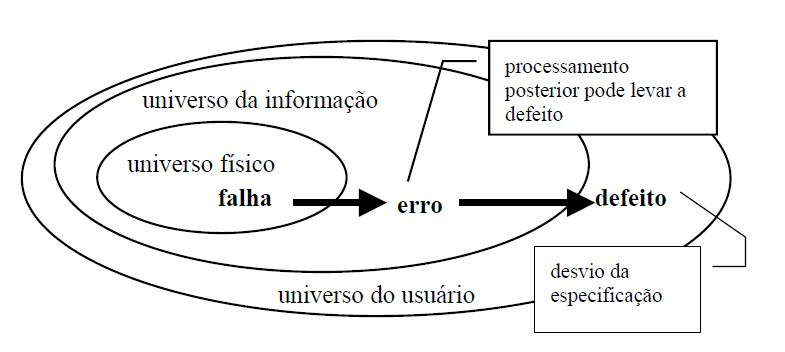
\includegraphics[width=0.7\textwidth]{figuras/modeloUniverso.jpg}
	\caption[Modelo de três universos]{Modelo de 3 universos: falha, erro e defeito. Retirado de Weber \cite{Weber:2002}.}
	\label{Img:modeloUniverso}	
	%width=0.5\textwidth (Tamanho da Imagem)
\end{figure}

Um exemplo de uma falha no universo físico é um chip de memória com uma falha do tipo grudado-em-zero (\textit{stack-at-zero}). Esta falha pode gerar um erro no universo da informação, uma vez que pode-se influenciar uma interpretação equivocada da informação armazenada em um dispositivo eletrônico, alterando o seu valor e como resultado esta alteração se torna um defeito, perceptível ao universo do usuário, no qual o sistema pode negar autorização de embarque para todos os passageiros de um voo \cite{Nelson:1990}. Na Figura \ref{Img:modeloUniverso} é mostrado a simplificação do exemplo anterior.

\section{Principais Fontes de Radiação e seus Efeitos nos Circuitos Eletrônicos} \label{sec:radiacao}

Em 1962 ocorreu uma falha no Satélite de Telecomunicações \textit{Telstar} após um teste nuclear realizado em alta altitude pelos Estados Unidos, surge então a primeira evidência de que a radiação pode perturbar a operação de circuitos eletrônicos \cite{Velazco:2007}. Após este acontecimento, a comunidade científica, agências espaciais e órgãos militares passaram a estudar os efeitos da radiação nos circuitos eletrônicos. Um segundo fato que levou a exploração desse assunto foi a queda de um avião Airbus A320 em fevereiro de 1990 na cidade de Bangalore na Índia, investigações preliminares sugeriram que os computadores de controle poderiam ter realizado algumas especificações segundos antes do início da queda \cite{LaprieAcidente:1990}.

A radiação está presente tanto no espaço quanto na atmosfera, podendo alterar a resposta ou danificar componentes eletrônicos expostos a íons pesados (partículas carregadas), como por exemplo, os transistores. Circuitos eletrônicos podem sofrer efeitos indesejados e as principais partículas responsáveis por isso são prótons, elétrons, nêutrons, íons pesados e partículas alfa, além da radiação eletromagnética (como, por exemplo, raio-x). As principais fontes de radiação de origem espacial são os cinturões de \textit{Van Allen}, os raios cósmicos \cite{Stassinopoulos:1988} e a atividade solar \cite{Boudenot:2007}. Estas partículas podem gerar pulsos transitórios nos transistores que dependendo de sua amplitude em tensão, corrente e duração podem ser interpretados como sinal interno do circuito, gerando erros. 


\subsection{Cinturão de Van Allen} \label{subsec: cinturao}

São imensas regiões de radiação dentro da magnetosfera repleta de prótons e elétrons energéticos presos pelo campo magnético da terra. Na Figura \ref{Img:cinturaoVanAllen} mostra-se dois cinturões de elétrons(interno e externo), sendo o cinturão externo o que contém partículas com maior energia. O cinturão interno contém elétrons cuja energia é menor que 5 MeV e pode ser encontrado numa região de aproximadamente 100 km a 10.000 km de altitude. Já o cinturão externo contém elétrons cuja energia pode alcançar até 7 Mev e situa-se em altitudes de aproximadamente 20.000 km até 60.000 km \cite{Stassinopoulos:1988}. Um terceiro cinturão de elétrons foi observado após uma tempestade magnética em 24 de março de 1991 \cite{Velazco:2007}.      

\begin{figure}
	\centering
	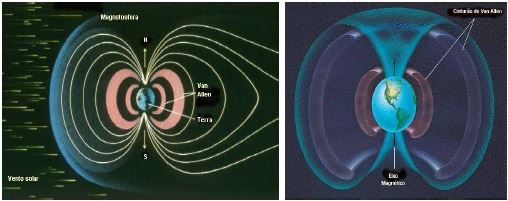
\includegraphics[width=0.7\textwidth]{figuras/cinturao.jpg}
	\caption[Cinturão de Van Allen]{Cinturão de Van Allen \cite{cinturao}.}
	\label{Img:cinturaoVanAllen}	
	%width=0.5\textwidth (Tamanho da Imagem)
\end{figure}

\subsection{Atividade Solar}

O sol é responsável por grande parte da radiação presente no espaço. A atividade solar segue uma variação regular e periódica com 11 anos de duração, e este período é comumente conhecido como ciclo solar. O ciclo solar é a recorrência de periódicas manchas solares na superfície do Sol. Durante o ciclo solar ocorre uma mudança periódica na energia solar, radiação e a ejeção de material solar \cite{Mansoori:2013}. O período de 11 anos correspondente ao ciclo solar está divido em aproximadamente 7 anos de alta atividade e 4 anos de baixa atividade \cite{Boudenot:2007}. 

Durante a baixa atividade solar o sol emite rajadas de partículas energéticas no espaço. Essas podem ser chamadas de erupções solares, que são compostas principalmente de prótons, com uma menor quantidade de partículas alfa (5\% a 10\%), íons pesados e elétrons, ou seja, as explosões solares emitem uma quantidade relativamente menor do que o fluxo de raios cósmicos que viajam pelo sistema solar.

Durante a alta atividade solar o sol emite uma quantidade maior de íons pesados podendo aumentar em até quatro ordens de grandeza, ou seja, o fluxo de íons é maior do que os observados para os raios cósmicos, por períodos que podem chegar a vários dias \cite{Stassinopoulos:1988}. 

A alta temperatura da coroa solar proporciona energia suficiente para que os elétrons escapem da atração gravitacional do sol. O efeito resultante da ejeção dos elétrons gera um desequilíbrio resultando numa ejeção de prótons e íons pesados da coroa solar. O vento solar é composto por aproximadamente 95\% de prótons, 4\% de íons de Hélio e 1\% de outros íons pesados e elétrons com uma quantidade necessária para tornar o vento solar neutro \cite{Velazco:2007}. 



\subsection{Raios Cósmicos} \label{subsec:raiosCosmicos}

O termo raio cósmico não possui uma definição científica clara. Ele tem sido utilizado desde o início do século XX para indicar as partículas energéticas que interferem com os estudos de materiais radioativos. Segundo Stassinopoulos e Raymond \cite{Stassinopoulos:1988} os raios cósmicos consistem em cerca de 85\% de prótons, cerca de 14 \% de partículas alfa, e cerca de 1\% de materiais mais pesados como, por exemplo, núcleo de carbono e ferro. Já Boudenot \cite{Boudenot:2007}, afirma que a composição dos raios cósmicos galácticos compreende 83\% de prótons, 13\% de núcleos de hélio e 3\% de elétrons. 

As Partículas produzidas na atmosfera da Terra surgem quando os raios cósmicos primários atingem átomos atmosféricos e criam uma chuva de partículas secundárias. Esses são também chamados de partículas em cascata. As partículas que finalmente atingem a terra são chamadas de partículas terrestres, menos de 1\% do fluxo primário atinge o nível do mar, e elas são na sua maioria compostas de múons, prótons, nêutrons e píons. A primeira observação de um \textit{Single Event Upset} (SEU) na superfície terrestre devido a raios cósmicos ocorreu no ano de 1979 \cite{ZieglerLandFord:1979}.


\subsection{Partículas alpha}

São compostas por dois nêutrons e dois prótons provenientes de um átomo de hélio duplamente ionizado a partir do decaimento nuclear de isótopos instáveis. No final da década de 70, as partículas alfa emitidas de materiais com traços de Urânio (U) e Tório (Th) foram mostradas como a causa dominante de um SEU numa memória \textit{RAM} na superfície terrestre \cite{Woods:1978}. Estas partículas estão presentes nos materiais utilizados para o encapsulamento de circuitos integrados, no qual é necessária uma baixa concentração de Urânio (U) e tório (Th) para reduzir a emissão e o equilíbrio de partículas alfa, mas não sendo o suficiente para eliminá-las. Em situações de não equilíbrio, foi destacado que o material utilizado no processo de solda dos dispositivos, usualmente feitos de cumbo (Pb) e estanho (Sn), os quais são extraídos de minérios que podem conter traços de Urânio (U) e Tório (Th) que causam a incidência de partículas alfa. Por isso é aconselhável que projetistas não posicionem pontos de solda próximos aos nós dos circuitos \cite{Velazco:2007}.


\subsection{Efeitos Singulares ou \textit{Single Event Effects}(SEE)} \label{subsec:EfeitosSingulares}

Efeitos singulares são causados por uma única partícula e podem assumir muitas formas. Estão associados a erros transientes num dispositivo causado pela indução de partículas energéticas ou radiação cósmica \cite{Yu:2008}. O impacto de uma única partícula ionizada da origem a pares de elétrons ao longo da trajetória da partícula por meio de um material semicondutor, SEE podem ser classificados em vários tipos como por exemplo:

\begin{itemize}
	\item \textit{Single Event Upsets}(SEU): Um SEU ocorre quando a incidência de uma partícula num dispositivo digital provoca mudanças indesejáveis no seu estado lógico, como por exemplo, a inversão de bits de elementos de memória. Esta inversão resulta de quando um pulso transitório incide num espaço de memória, esse efeito é visto como uma inversão do valor de armazenamento no \textit{flip-flop}, ou seja, um \textit{bit-flip} \cite{Normand:1996}.
	
	\item \textit{Single Event Transients}(SET): São variações temporárias na tensão de saída de corrente ou de um circuito
	devido à passagem de um íon pesado através de um dispositivo sensível, ou seja, pulso transiente que pode ou não ser capturado por um elemento de memória \cite{Ecoffet:1994}.
\end{itemize}

\section{Dependabilidade} \label{sec:denpendabilidade}

Segundo Laprie \cite{LaprieAcidente:1990}, dependabilidade indica a qualidade do serviço fornecido por um dado sistema e a confiança depositada no serviço fornecido. Do ponto de vista etimológico ao que diz respeito ao termo dependabilidade, do inglês \textit{dependability}, o termo confiabilidade, do inglês \textit{reability} seria mais apropriado: a capacidade de confiar. Apesar de que \textit{dependability} é sinônimo de \textit{reability} \cite{LaprieAcidente:1990}. 

Segundo Laprie e Weber \cite{LaprieAcidente:1990, Weber:2002} tolerância a falhas e dependabilidade não são propriedades de um sistema a que se possa atribuir diretamente valores numéricos. Mas todos os atributos da dependabilidade correspondem a medidas numéricas. Seus principais atributos são dependabilidade, confiabilidade, disponibilidade, segurança de funcionamento (\textit{safety}) e segurança (\textit{security}). Um resumo dos principais
atributos é mostrado na Tabela \ref{Img:atDenp}.     


\begin{table}[h]
	\centering
	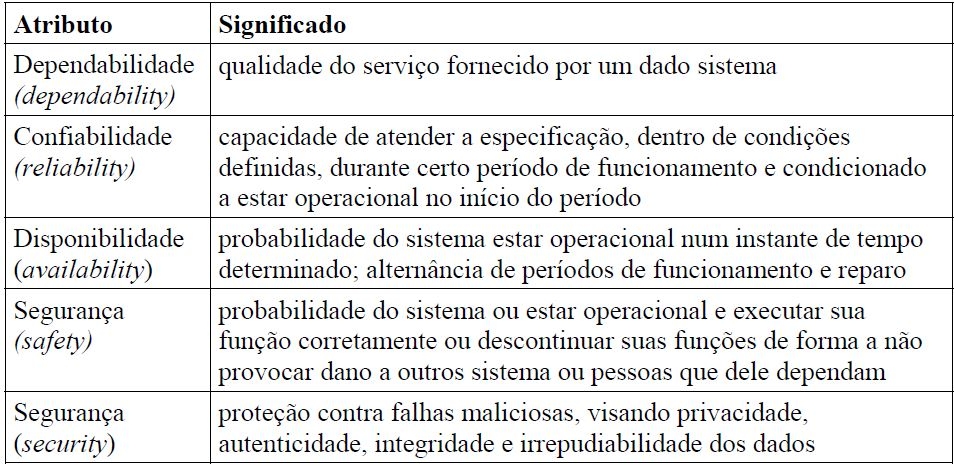
\includegraphics[width=0.7\textwidth]{figuras/tabelaDenpendabilidade.jpg}
	\caption[Resumo dos Atributos de Denpendabilidade]{Resumo dos atributos de dependabilidade Retirado de Weber \cite{Weber:2002}.}
	\label{Img:atDenp}	
	%width=0.5\textwidth (Tamanho da Imagem)
\end{table}



\section{Tolerância a Falhas} \label{sec:tolerancia}

Segundo Avizienis \cite{Avizienis:1984} quando um sistema é capaz de automaticamente se recuperar de erros causados por falhas, e eliminar uma falha sem sofrer um defeito externamente perceptível, diz-se que este sistema é tolerante a falhas. Na construção dos primeiros computadores, estratégias para construção de sistemas mais confiáveis já eram utilizadas para tolerar possíveis falhas \cite{VonNewmann:1956}. Apesar de envolver técnicas e estratégias tão antigas, a tolerância a falhas ainda não é uma preocupação rotineira de projetistas e usuários, ficando sua aplicação quase sempre restrita a sistemas críticos e mais recentemente a sistemas de missão crítica \cite{Weber:2002}.

Um aspecto importante em tolerância a falhas é a descrição das características das falhas. Há um conjunto de atributos que são utilizados para cumprir esta finalidade; são eles: causa, natureza, duração, extensão e valor. Na figura \ref{Img:falhasCaracteristicas} é mostrado os atributos das características das falhas.

Pêgo \cite{Pego:2014} descreve os conjuntos de atributos utilizados para caracterizar uma falha:

\begin{figure}[H]
	\centering
	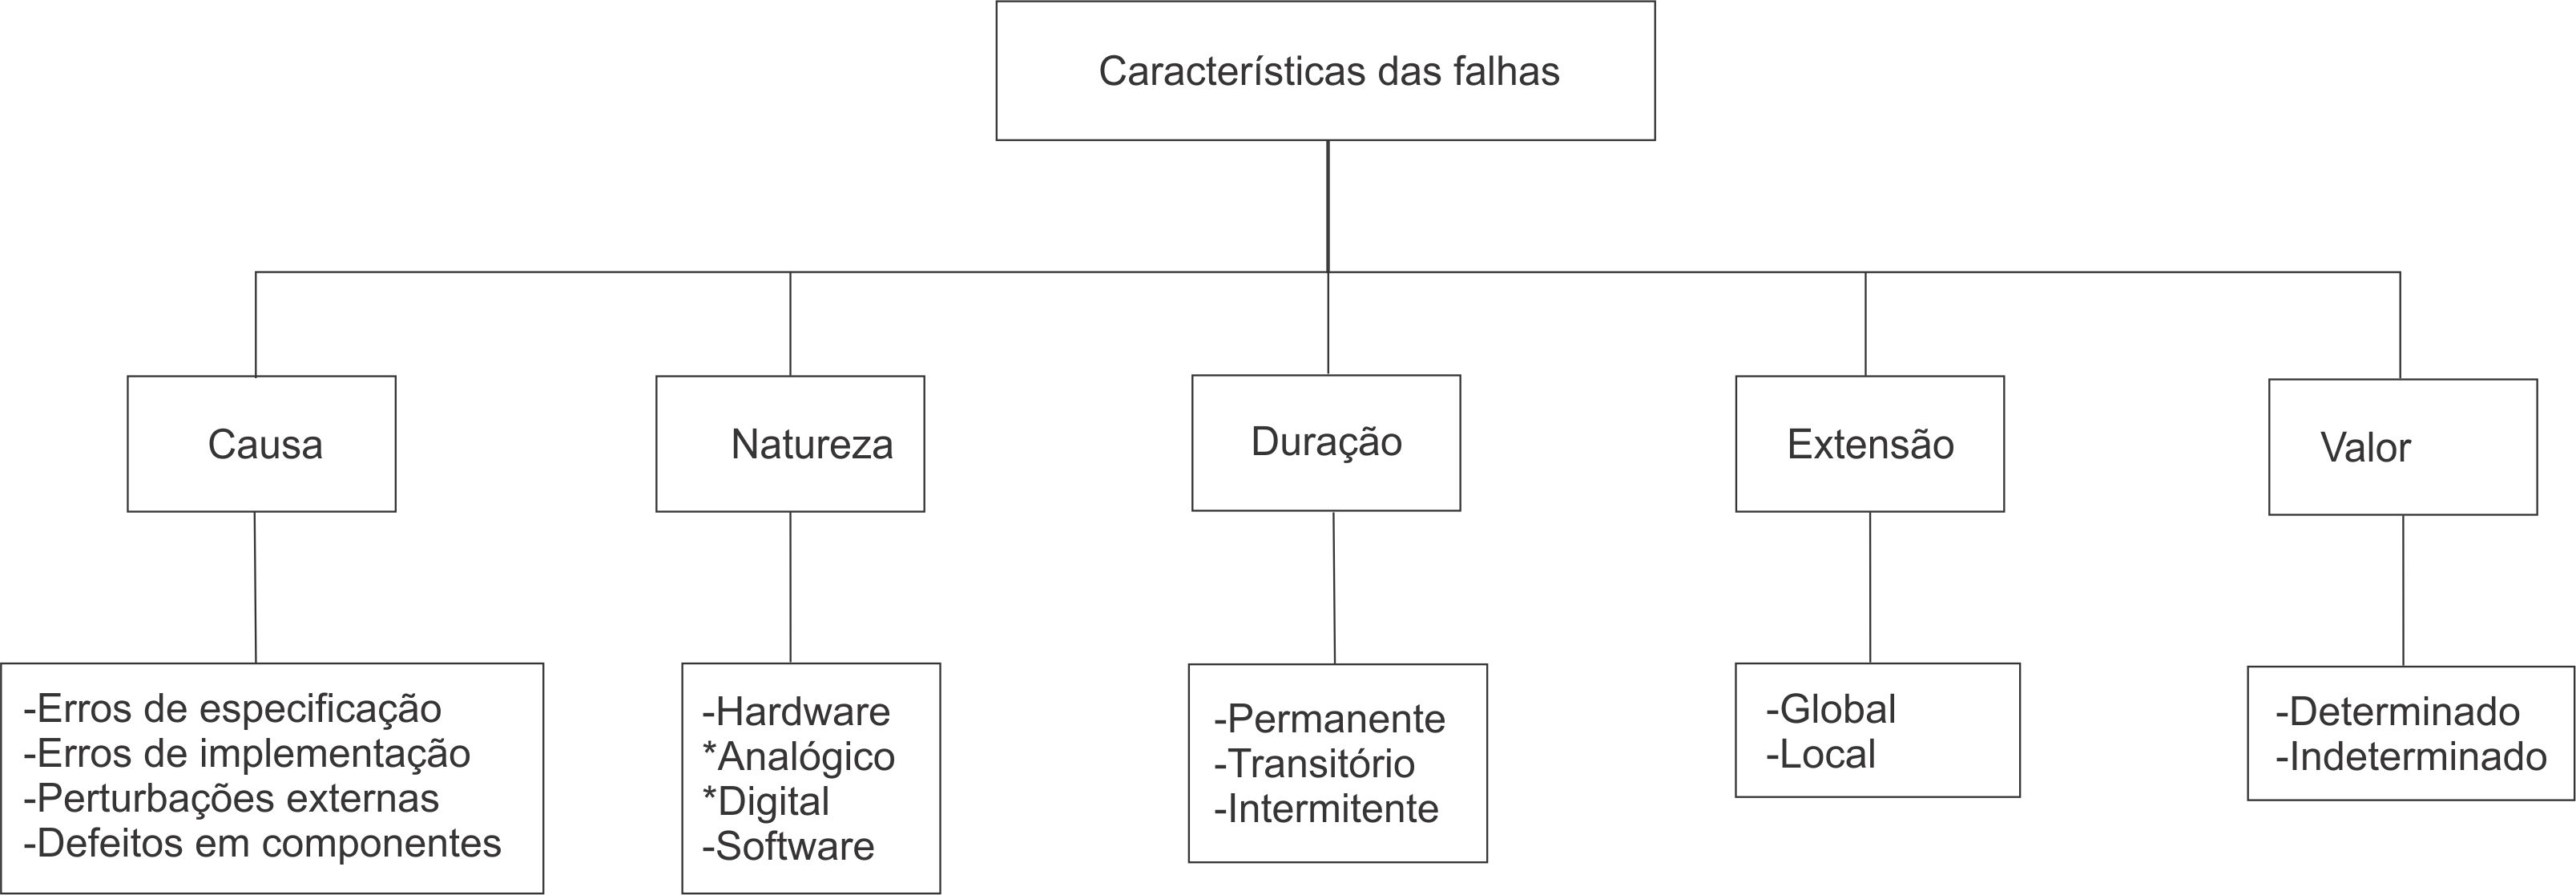
\includegraphics[width=0.7\textwidth]{figuras/falhasCaracteristicas.jpg}
	\caption[Características das Falhas]{Atributos das características das falhas. Retirado de Pego \cite{Pego:2014}.}
	\label{Img:falhasCaracteristicas}	
	%width=0.5\textwidth (Tamanho da Imagem)
\end{figure}

\begin{itemize}
	\item \textbf{Causa} - Uma falha pode ter origem em problemas de especificação, problemas de execução, defeitos em componentes do sistema operacional (que não são incomuns para dispositivos eletrônicos), ou em fatores externos, tais como, tempestades, poeira, temperatura, etc.
	
	\item \textbf{Natureza} - Uma falha pode ser proveniente de \textit{software} ou \textit{hardware}. Neste último, a falha pode estar na parte analógica, por exemplo, em transdutores e amplificadores, ou na parte digital, por exemplo, na unidade lógica Aritmética (ULA).
	
	\item \textbf{Duração} - Uma falha pode ser constante, o que significa que uma vez que os dados tenham sido persistidos no sistema, a falha continuará até que a manutenção adequada seja feita. Pode ainda ser transitória, quando ocorre em um período de tempo e logo em seguida, desaparece. Esse tipo de falha é geralmente provocada por causas externas. Relâmpago, por exemplo, podem provocar um erro súbito em um dispositivo, mas após o relâmpago, o dispositivo voltará ao seu funcionamento normal. Finalmente, há falhas, que são chamadas intermitentes; essas ocorrem em períodos curtos de tempo e desaparecem, mas depois elas voltam novamente. É possível que este processo se repita indefinidamente. Uma falha intermitente é a ocorrência de repetição de falhas transitórias.
	
	\item \textbf{Extensão} - A ocorrência de uma falha pode estar limitada a um escopo global ou local. Ou seja, uma falha pode afetar todo o sistema ou ser limitada a um determinado bloco. 
	
	\item \textbf{Valor} - O valor de uma falha pode ser determinado ou indeterminado. Ou seja, os valores relativos de uma falha podem ser constantes ou não. Na Seção \ref{sec:falhaErroDefeito} é citado um exemplo de uma falha que mantém um endereço de memória com um valor fixo em zero, este exemplo é chamado de valor determinado. Outra falha sem esta característica é chamada de indeterminada.
	
	
	
\end{itemize}


\section{Técnicas de Tolerância a Falhas}\label{sec:tecnica}

Para mitigar(abrandar, minimizar) os efeitos citados na Subseção \ref{subsec:EfeitosSingulares} e na Seção \ref{sec:falhaErroDefeito} são utilizadas técnicas de tolerância a falhas, nas quais envolvem alguma forma de redundância.  
Existem técnicas baseadas em \textit{software} e \textit{hardware}, neste trabalho foram citados apenas as técnicas baseadas em \textit{software}, pois no desenvolvimento da aplicação proposta não foram utilizadas as técnicas baseadas em \textit{hardware}, pois esta técnica demanda da utilização de um equipamento que realiza o bombardeamento de íons sobre o circuito eletrônico podendo danificar o \textit{hardware} \cite{Weber:2002}.

\subsection{Técnicas de redundância baseadas em software}

Segundo Pêgo \cite{Pego:2014} a inserção de redundância no código ou nos dados permite que seja possível detectar e até mesmo corrigir eventuais falhas. A inserção de instruções pode ser feita em programas escritos tanto em liguagem C, \textit{assembly} e até em níveis mais baixos, a redundância temporal em nível de intruções pode ser dividida em:


\begin{itemize}
	\item \textbf{Técnicas orientadas a dados} - Cada dado armazenado é replicado em cada operação, na checagem da consistência dos dados sendo necessária a alteração do código fonte. Pode ser implementado em linguagens de baixo nível como C, que será utilizada neste trabalho, \textit{assembly} e até no código intermediário gerado pelo compilador \cite{Pego:2014}.
	
	\item \textbf{Técnicas orientadas ao controle} - As falhas que podem modificar o fluxo correto de execução dos programas são detectadas e tratadas. Todas as técnicas no nível de instrução são baseadas na divisão do código do programa em blocos, construção de grafos e a checagem em tempo de execução sobre a correta transição entre os vértices deste grafo \cite{Pego:2014}.  		 
	
\end{itemize}


Weber \cite{Weber:2002} afirma que a simples replicação de componentes idênticos é uma estratégia de detecção e mascaramento de erros inútil em \textit{software}. Componentes idênticos de \textit{software} vão apresentar erros idênticos. Assim não basta copiar um programa e executá-lo em paralelo ou executar o mesmo programa duas vezes em tempos diferente. Erros de programas idênticos vão apresentar, com grande probabilidade, de forma idêntica para os mesmos dados de entrada. Segundo Brilliant \textit{et al.}\cite{Brilliant:1990} outras formas de redundância de \textit{software} como, por exemplo, diversidade ou programação n-versões, blocos de recuperação e variação de consistência não envolvem cópias idênticas.

\subsection{Diversidade ou Programação N-Versões}

A partir de um problema, são implementadas diversas soluções alternativas, sendo a reposta do sistema determinada por votação, esta técnica é ilustrada na Figura \ref{Img:nVersion}. Segundo Avizienis \cite{Avizienis:1995} A. \textit{apud} Fischler et. al., os esforços de programação são realizados por \textit{n} indivíduos. Sempre que for possível, diferentes algoritmos e linguagens de programação são usados em cada versão. Cada versão do programa é implementada de forma independente com base na especificação inicial do problema, embora sejam diferentes na sua implementação, as N-versões são funcionalmente equivalentes e dificilmente apresentarão as mesmas falhas \cite{Avizienis:1995}. 

\begin{figure}[H]
	\centering
	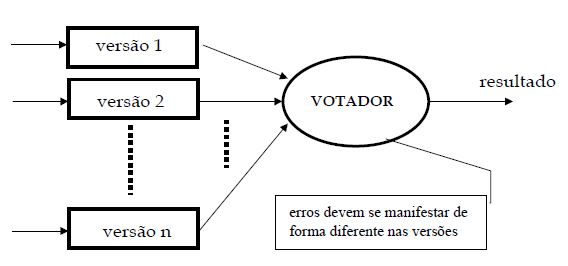
\includegraphics[width=0.7\textwidth]{figuras/nVersions.jpg}
	\caption[Programação N-Versões]{Diversidade ou Programação N-Versões. Retirado de Weber \cite{Weber:2002}.}
	\label{Img:nVersion}	
	%width=0.5\textwidth (Tamanho da Imagem)
\end{figure}  

Um exemplo de programação n-versões é o sistema de bordo do \textit{Space Shutle}, no qual quatro computadores idênticos são utilizados em NMR (\textit{N-Modular Redundancy}). Esta técnica consiste em replicar o \textit{hardware} responsável pelo processamento da informação em \textit{n} módulos. Um quinto computador com \textit{hardware} diferente dos outros quatro, pode substituir os demais em caso de colapso no esquema NMR \cite{Pradhan:1996}.

\subsection{Blocos de Recuperação}

Nesta técnica são utilizados testes de aceitação, no qual programas serão executados um a um até que o primeiro passe no teste de aceitação. A técnica de blocos de recuperação é semelhante a programação n-versões, mas nessa técnica programas secundários só serão necessários na detecção de um erro no programa primário. Esta técnica tolera n-1 falhas, no caso de falhas independentes nas \textit{n} versões \cite{Nelson:1990, Weber:2002, Somani:1997}.   

\begin{figure}[H]
	\centering
	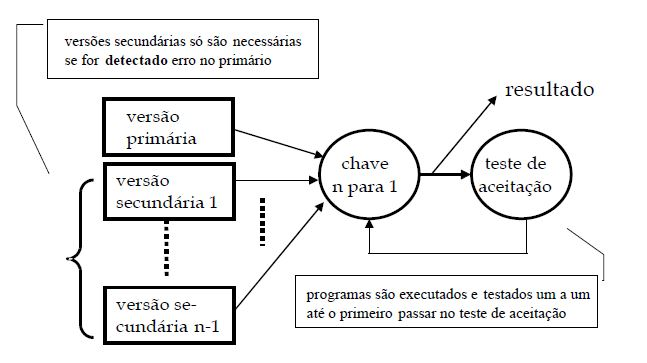
\includegraphics[width=0.7\textwidth]{figuras/blocoRecuperacao.jpg}
	\caption[Blocos de Recuperação]{Blocos de Recuperação. Retirado de Weber \cite{Weber:2002}.}
	\label{Img:blocoRecuperacao}	
	%width=0.5\textwidth (Tamanho da Imagem)
\end{figure}


\subsection{Verificação de Consistência}

É uma ampliação da programação n-versões. Nessa técnica também são utilizadas \textit{n} equipes, assim como na programação n-versões, que implementam soluções independentes a partir de uma única especificação, no entanto, as equipes também desenvolvem um módulo específico para verificar a saída dos dados de seu próprio sistema em tempo real e compará-los com uma base de informações prévia para apurar a corretude da informação. Os \textit{softwares} das equipes são executados paralelamente e as saídas são submetidas a verificação. A saída passa a ser verificada em seu próprio módulo e o resultado é definido pelo primeiro módulo que passar ou por um sistema de votação \cite{Nelson:1990,Kruger:2014}.

\section{Injeção de Falhas} \label{sec:InjecaoDeFalhas}

A injeção de falhas é um processo importante para validar e verificar a confiabilidade de um sistema, seja por alteração de código, simulando uma falha de \textit{software} \cite{Kanawati:1995} ou a nível de pinos (\textit{Pin-level Injection}) injetando falhas diretamente no \textit{hardware} \cite{Arlat:2003}. Além da injeção de  falhas por \textit{software} e por \textit{hardware} existe um terceiro tipo chamado injeção de falhas por Simulação. Arlat \cite{Arlat:2003} afirma que injeção de falhas baseadas em simulação se restringem aos modelos de alto nível, como por exemplo os modelos VHDL (\textit{VHSIC Hardware Description Language}) Linguagem de descrição de \textit{hardware} de circuitos de alta velocidade. 

Segundo Arlat \textit{et. al.} \cite{Arlat:1990} a validação e auxílio de projeto são as duas metas principais que compõem o método de injeção de falhas. Com um conjunto de testes a validação dos procedimentos de verificação são utilizados para descobrir falhas durante todo o processo de desenvolvimento. A validação dos mecanismos de tolerância a falhas é usada para detecção e recuperação de falhas com o objetivo de alcançar a dependabilidade do sistema na fase operacional. É importante ressaltar dois aspectos importantes na validação, que é a previsão de falhas, na qual os mecanismos de manipulação de falhas são avaliados em sua eficiência na estimação de medidas como cobertura e latência \cite{Arlat:1990}.

O auxílio ao projeto ocorre durante a fase de desenvolvimento do projeto, buscando melhorar a eficiência dos mecanismos de testes e o protocolo de tolerância a falhas por meio da injeção de falhas \cite{Arlat:1990}.

Uma das vantagens da utilização do método de injeção de falhas está no fato de ser uma técnica que permite a avaliação de um protótipo de sistema sob falhas, em particular ela mede a eficácia da detecção de erros do sistema e sua capacidade de correção. Outra vantagem são os efeitos das falhas no sistema que permitem revelar falhas críticas que por ventura viessem a ocorrer na execução do sistema em um ambiente real \cite{Arlat:2003}.     

\subsection{Injeção de falhas por \textit{Hardware}}

Esta técnica necessita de um \textit{hardware} especial, no qual as falhas seriam originadas. Arlat \cite{Arlat:2003} apresenta algumas ferramentas para injeção de falhas por \textit{hardware} como \textit{MESSALINE}, \textit{RIFLE} E \textit{AFIT}, todas utilizadas para injeção de falhas a \textit{pin-level}, que consiste na injeção de falhas por meio de pinças ou posicionando o circuito sobre soquetes conectados a um injetor de falhas \cite{Arlat:1990, Arlat:2003}. Outras técnicas de injeção de falhas por \textit{hardware} são interferências eletromagnéticas e irradiação de íons pesados \cite{Gunnelo:1989, Arlat:1990, Arlat:2003}, estas por sua vez podem danificar o componente sob teste \cite{Sotoma:1997}. O objetivo dessas técnicas visa principalmente estudar o comportamento dos mecanismos de tolerância a falhas implementados por \textit{hardware}, porém também se pode testar os mecanismos de falhas por meio de \textit{softwares} que não danificam os componentes sob teste \cite{Martins:1989}.


\subsection{Injeção de falhas por \textit{Software}}

Esta técnica visa modificar o estado do \textit{hardware/software} do sistema por meio de um programa, fazendo com que o sistema se comporte como se uma falha de \textit{hardware} estivesse ocorrendo. Pode-se emular falhas em vários níveis do sistema desde que a funcionalidade do \textit{hardware} esteja visível através do \textit{software}. Por isso, injetar falhas por \textit{software} é menos dispendioso em termos de tempo e esforço do que as técnicas de \textit{hardware} implementadas, devido a capacidade de alterar o estado de registradores e memória \cite{Kanawati:1995}. Um exemplo de injeção de falhas por \textit{software} é a ferramenta \textit{Ferrari} apresentada por Kanawati \textit{et. al.} \cite{Kanawati:1995} que possibilita a injeção de falhas transitórias, bem como falhas permanentes, de modo que ele possa verificar a eficácia da detecção de erros e a correção simultânea dos mecanismos de verificação de falhas, e a capacidade para executar a injeção em código aberto. Alguns exemplos de injetores de falhas são FERRARI \cite{Kanawati:1995}, PFI \cite{Dawson:1995}, SFI \cite{Rosenberg:1993} e FIAT \cite{Segall:1988}. 


\section{\textit{Design Patterns}} \label{sec:designPattern}
				
Neste trabalho foi necessário a utilização de \textit{design patterns} (padrões de projeto) para a elaboração de códigos eficientes. A ideia básica dos padrões de projeto é a de utilizar soluções conhecidas para problemas conhecidos. Cada padrão de projeto descreve um problema e sua solução, com isso, terceiros podem a utilizar sem ter a necessidade de descobri-la novamente, economizando tempo e padronizando o desenvolvimento do projeto \cite{Vinicius:2009}. Em geral, \textit{design patterns} possuem alguns elementos que facilitam no desenvolvimento da sua aplicação \cite{Engholm:2010}, são eles:

\begin{itemize}
	\item \textbf{Contexto} - Situação na qual o problema está sendo endereçado corretamente.
	
	\item \textbf{Problema} - Problema de design para o qual o padrão se destina.
	
	\item \textbf{Necessidade} - Quesitos de design para o qual o padrão se destina.
	
	\item \textbf{Solução e estrutura} - Solução do problema.
	
	\item \textbf{Consequências} - Vantagens e desvantagens de se utilizar o padrão.
	
	\item \textbf{Padrões associados} - Padrões similares ou utilizados para construir o padrão.
\end{itemize}

\subsection{Padrão GoF (Padrões Fundamentais Originais)} \label{subsec:gof}

O conceito de máquina de estados foi utilizado neste trabalho  para o desenvolvimento da biblioteca \textit{FaultRecovery}. O padrão \textit{State} vai ao encontro da resolução deste problema.

Os padrões GoF são divididos em três grupos: padrões de comportamento, de criação e estruturais. Estes descrevem como os objetos devem ser gerenciados pelas estruturas de um programa, esses fornecem maneiras robustas de se criar objetos, e aqueles descrevem como os objetos interagem, distribuindo responsabilidades \cite{Engholm:2010}. Neste trabalho utilizou-se o padrão \textit{State}, indicado para programas que podem ser representados por uma máquina de estados, que é o caso dos \textit{firmwares} desenvolvidos para o microcontrolador \textit{mbed}. O padrão \textit{State} faz parte dos padrões de comportamento e permite que parte do comportamento de um objeto seja alterado conforme o estado do objeto. Cada objeto possui atributos, que representam seu estado, e também métodos, que representam seu comportamento \cite{Vinicius:2009}. % Fundamentação
	%====================================================================================================
%----------------------------------------------------------------------------------------------------
% Autor				: Vagner da Silva Bezerra
%----------------------------------------------------------------------------------------------------
% Data de criação	: 10 de Outubro de 2016
%====================================================================================================

\chapter{Metodologia} \label{cap:metodologia}

%Devido ao fato de haver bibliotecas que não passaram por nenhum tipo de teste de desempenho ou de funcionalidade. Ocorre muitas das vezes a existência de fahas causadas por leaks de memória, por exemplo, a biblioteca ConfigFile baixada do repositório do mbed. Essas falhas pode ser detectada pela ferramenta valgrind. Leaks de memória: invalid free, invalid write e invalide read. Citar dissertação Kleber.

Este trabalho teve como objetivo ampliar as bibliotecas \textit{FaultInjector} e \textit{FaultRecovery}, ambas desenvolvidas por Kruger \cite{Kruger:2014} em sua dissertação de mestrado. A biblioteca \textit{FaultInjector} possibilita a injeção de falhas no sistema mediante a simulação do fenômeno \textit{bit-flip} nas regiões da memória \textit{SRAM} do microcontrolador. Já a biblioteca \textit{FaultRecovery} proporciona o desenvolvimento de sistemas embarcados confiáveis, pois dispõe de técnicas de tolerância a falhas (baseadas na redundância de dados e de processamento) para aumentar a confiabilidade do sistema.

Foram utilizados exemplos variados para exemplificar as modificações realizadas na \textit{FaultRecovery}, pois se pensou em criar uma biblioteca genérica que possa ser utilizada em diversos casos, seja no sistema embarcado (\textit{firmware}) de um estacionamento, em um robô seguidor de linha ou em uma estação meteorológica.

%Como expansão ao trabalho de Kruger, foi melhorado o injetor de falhas de falhas na memória \textit{flash} da biblioteca \textit{FaultInjector} e a classe TData, responsável pela redundância de dados. A arquitetura da biblioteca também pode ser utilizada por sistemas de outras plataformas, por exemplo, os sistemas embarcados implementados para \textit{arduino} que são utilizados na área de robótica e são implementados por meio de máquina de estados.

Para a ampliação das biblioteca citadas, utilizou-se um microcontrolador de prototipagem rápida \textit{mbed}, modelo NXP LPC1768 \cite{lpc1768:2016} (o mesmo utilizado por Kruger). Este é projetado para a prototipagem de diversos equipamentos, especialmente aqueles que necessitam de conexão com a internet, portas USB e interfaces variadas para periféricos. Ele possui um núcleo ARM Cortex-M3 32 bits com 96 MHz de \textit{clock}, 64 KB de memória \textit{RAM} (32 KB disponíveis ao usuário e 32 KB reservados aos controladores internos do dispositivo), uma memória \textit{flash} de 512 KB, portas \textit{built-in Ethernet}, USB Host, CAN (\textit{Controller Area Network}), SPI (\textit{Serial Peripheral Interface}), I2C (\textit{Inter-Integrated Circuit}), ADC (\textit{Analog-to-Digital Converter}), DAC (\textit{Digital-to-Analog Converter}), PWM (\textit{Pulse-Width Modulation}) e outras interfaces de entrada e saída.

O \textit{mbed} também possui um temporizador \textit{watchdog}. Este componente consiste em um hardware responsável por reiniciar automaticamente o dispositivo em caso de falhas. O hardware temporizador é carregado com um valor inicial, decrementado a cada vez que o \textit{watchdog} é executado. Enquanto isso o programa principal executa em um \textit{loop}, repondo o temporizador a cada vez que passa pelo circuito principal. Se por conta de uma falha a reposição não ocorrer e o temporizador zerar, o dispositivo é reiniciado \cite{mbedWhatdog:2016}.

No sítio oficial da plataforma \textit{mbed} são fornecidas soluções para auxiliar no desenvolvimento de sistemas embarcados. Além da possibilidade de baixar bibliotecas fornecidas pela comunidade, o sítio disponibiliza um \textit{forum} para retirada de dúvidas. A \textit{mbed} também fornece um compilador online, com o qual após a compilação do código, um arquivo binário é gerado para ser executado no microcontrolador. Este compilador online tem a capacidade de compilar códigos para diversos modelos do \textit{mbed} \cite{mbedCompiler:2016}.

Além do modelo LPC1768, existem outros pertencentes à família \textit{mbed} NXP LPC17X, são eles: LPC1764, LPC1765, LPC1766 \cite{manualLpc176x:2016}. Embora apresentem arquiteturas compatíveis, o tamanho e o mapa de memória \textit{flash} e \textit{SRAM} varia conforme cada modelo, distinguindo-se por exemplo, nos modelos LPC1768/66/65 que possuem regiões de memória \textit{SRAM} nas mesmas faixas de endereço, mas diferentes do modelo LPC1764, conforme é mostrado na Figura \ref{Img:memoryMap} da seção a seguir.

%Nenhuma outra técnica, além do temporizador \textit{watchdog} foi utilizada para aumentar a confiabilidade do sistema \cite{Kruger:2014}.O Compilador online foi utilizado neste trabalho para criar a arquitetura para o desenvolvimento. Com o primeiro contato com o microcontrolador \textit{mbed} identificou-se a necessidade de estudar suas funcionalidades. Com a utilização do compilador online foi possível verificar que seria inviável adotá-lo como um editor de código para a expansão do injetor de falhas e da biblioteca \textit{faultRecovery}. A solução encontrada foi a utilização do ambiente de desenvolvimento integrado (IDE) LPCXpresso, pois o compilador online do \textit{mbed} permite exportar a arquitetura criada para essa IDE. O LPCXpresso é baseado na IDE eclipse e possui versões gratuitas e pagas, neste trabalho utilizou-se a versão gratuita para o modelo NXP LPC176. 

%, implementando um mapeamento do espaço de memória permitindo com que o injetor de falhas possa ser utilizado por qualquer modelo \textit{mbed} LPC176x, injeção de falhas na memória \textit{flash} e a ampliação da biblioteca \textit{faultRecovery} para implementação de sistemas embarcados por meio de máquinas de estados.

%Nenhuma outra técnica, além do temporizador \textit{watchdog} foi utilizada para aumentar a confiabilidade do sistema \cite{Kruger:2014}. dissertação de mestrado de Kruger \cite{Kruger:2014} o módulo \textit{GPS} não enviava dados para o servidor, sabendo-se que o microcontrolador \textit{mbed} pode se conectar a internet por meio desse módulo, a funcionalidade para enviar os dados coletados pela estação meteorológica será implementada nos próximos meses de execução deste trabalho, atualmente a biblioteca \textit{GPS} está com um erro de programação que fixa a execução do código em um loop infinito.


\section{Injetor de Falhas} \label{sec:InjetorDeFalhas}

A injeção de falhas é um processo importante para validar e verificar a confiabilidade de um sistema, seja por alteração de código, simulando uma falha de \textit{software} ou a nível de pinos (\textit{Pin-level Injection}), injetando falhas diretamente no hardware. A biblioteca \textit{FaultInjector} permite simular o efeito do \textit{bit-flip} em qualquer região de memória \textit{SRAM} do microcontrolador \textit{mbed} LPC1768, mas apresenta duas graves limitações: a falta de flexibilidade, por não executar em outros modelos de microcontroladores, e a impossibilidade de inserção de falhas nas regiões da memória \textit{flash}. Essas limitações são descritas respectivamente nas subseções \ref{subsec:MapDeMemoria} e \ref{subsec:InjecaoFalhasFlash}.

\subsection{Mapeamento de Memória} \label{subsec:MapDeMemoria}

Inicialmente, pensou-se em ampliar o uso da biblioteca \textit{FaultInjector} mediante a criação de várias versões, cada uma específica a um modelo da família LPC176X. Assim, o programador ficaria responsável por baixar a versão correta. Entretanto, conforme as pesquisas evoluíram, percebeu-se que era possível identificar dentro do próprio código-fonte o modelo do microcontrolador, uma vez que o compilador mantém a informação do modelo em uma \textit{define} \footnote{Constante}. Com esta descoberta, foi possível criar uma única versão que automaticamente mapeia as regiões de memória.

Neste primeiro passo, observando o mapa de memória da família \textit{mbed} LPC176X \cite{manualLpc176x:2016} foi possível constatar que alguns modelos possuem regiões de memória idênticas, conforme mostrados na Figura \ref{Img:memoryMap}. Logo, o uso de heranças e classes abstratas poderiam ser utilizadas com o intuito de facilitar o mapeamento das regiões de memória e promover uma interface à biblioteca \textit{FaultInjector}, que precisava injetar falhas nas regiões de memória sem necessariamente conhecer os endereços das regiões de cada dispositivo.

Com as regiões de memória mapeadas, o segundo passo foi a implementação desse mapeamento. A classe \textit{MemoryRegion}\cite{Kruger:2014} foi utilizada para representar as regiões de memória do \textit{mbed}. Ela contém atributos que armazenam o endereço de memória inicial, o endereço final e o tamanho (em bytes) de cada região de memória. 

A classe abstrata \textit{MemoryMap} representa o mapa de memória de um microcontrolador \textit{mbed} e disponibiliza uma interface para \textit{FaultInjector} injetar falhas. Esta classe é herdada por classes não-abstratas, como a classe \textit{MemoryMap\_LPC1764} e \textit{MemoryMap\_LPC1768}, que obrigatoriamente, ficam responsáveis por implementar os métodos abstratos \textit{getUserMemoryRegion()} e \textit{getFlashMemoryRegion()} de \textit{MemoryMap}, descritos a seguir:

\begin{itemize}
	\item \textbf{\textit{getUserMemoryRegions()}} - método abstrato que retorna uma lista das regiões de memória disponíveis para o usuário.				
	
	\item \textbf{\textit{getFlashMemoryRegions()}} - método abstrato que retorna a lista de regiões endereçadas a memória \textit{flash}.
	
	\item \textbf{\textit{getPeripheralsMemoryRegions()}} - retorna uma lista de regiões da memória destinadas aos periféricos. Este método não é abstrato, mas pode ser sobrescrito. Entretanto, como as regiões dos periféricos do microcontrolador é comum a todos eles, não há necessidade alguma sobrescrever este método.
\end{itemize}

Pela \textit{FaultInjector} ser capaz de identificar o modelo do microcontrolador, ela mesma é responsável por escolher qual das versões de \textit{MemoryMap} irá utilizar (\textit{MemoryMap\_LPC1764}, \textit{MemoryMap\_LPC1765}, entre outros). Isso tornou a biblioteca flexível, sendo possível injetar falhas nos nas regiões de memória mostradas na Figura \ref{Img:memoryMap}. A biblioteca está disponível no endereço \url{https://github.com/cleitonalmeida1/FaultInjector}.

\begin{figure}[H]
	\centering
	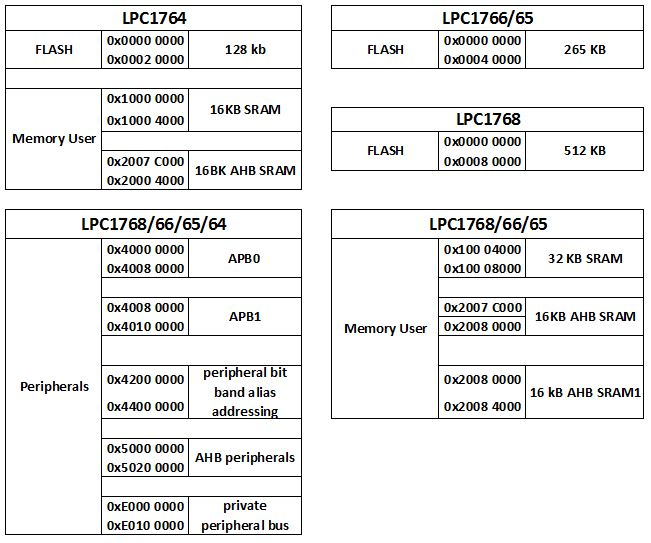
\includegraphics[width=1.0\textwidth]{figuras/memoryMap.jpg}
	\caption[Mapas das Regiões de Memória dos Modelos LPC1768/66/65/64]{Mapeamento das regiões de memória dos modelos LPC1768/66/65/64.}
	\label{Img:memoryMap}	
	%width=0.5\textwidth (Tamanho da Imagem)
\end{figure}


\subsection{Injeção de Falhas na Memória Flash} \label{subsec:InjecaoFalhasFlash}

Os microcontroladores \textit{mbed} possuem memória \textit{flash}, na qual o código do \textit{firmware} é armazenado \cite{manualLpc176x:2016}. Logo, a alteração de um único bit em um endereço de memória que contenha partes de uma instrução pode resultar em um falha irreversível. No entanto os dados coletados por um sistema também podem ser armazenados na memória \textit{flash}. Considerando-se o sistema embarcado de uma estação meteorológica que precisa coletar os dados climáticos e armazená-los na memória não volátil. Estes dados armazenados na \textit{flash} são enviados a um servidor remoto após um período de tempo predefinido. Se um único bit da região de memória na qual os dados coletados estão armazenados for alterado (\textit{bit-flip}), esta alteração poderá provocar uma modificação no valor da informação armazenada que poderia ser, por exemplo, um valor da umidade do ar, que perderia a exatidão após sua alteração, ou seja, o dado coletado enviado para o servidor remoto estaria incorreto, impactando em uma equivocada previsão do tempo. 

Conforme explicado na Seção \ref{sec:InjecaoDeFalhas}, um dos aspectos positivos na simulação de falhas por software é a segurança de não danificar o dispositivo. Falhas podem ser inseridas em bytes aleatórios na memória \textit{SRAM} simulando o fenômeno \textit{bit-flip}, entretanto, a mesma lógica não pode ser aplicada na memória \textit{flash}, pois por ser protegida não é possível escrever um único endereço de memória, somente a escrita por setores que são no total 29, divididos em duas áreas. A primeira, que abriga os setores do 1 ao 15 contém blocos de 4KB, a segunda, que vai do setor 16 até o 29, é composta por blocos de 32KB para cada setor \cite{manualLpc176x:2016}.

A injeção de falhas na \textit{flash} foi realizada mediante a escrita de bytes em um setor de memória sorteado aleatoriamente. Foram copiado 256 bytes da memória \textit{SRAM}, que é a quantidade mínima de bytes que podem ser escritos com a biblioteca retirada do repositório de bibliotecas da \textit{mbed} \cite{escritaNaFlash:2016}, para a \textit{flash} utilizando uma biblioteca que permite fazer operações na memória não volátil. 

Para realizar a injeção de falhas na flash foi necessário seguir os seguintes passos:

\begin{itemize}
	\item Sortear um setor aleatório da memória flash.
	
	\item Copiar a quantidade de bytes escolhida da memória \textit{RAM} podendo variar entre 256, 512, 1024 ou 4096.
	
	\item Preparar o setor para escrever os bytes copiados da memória \textit{RAM} determinando qual o número do setor inicial e qual o do setor final.
	
	\item Após a delimitação do setor inicial e final a escrita dos bytes copiados da memória serão escritos na flash.
	
\end{itemize}

Neste trabalho foi realizada a escrita de 256 bytes na memória \textit{flash}, ou seja, foram injetadas 256 bytes de falhas em setores aleatórios. As regiões da \textit{flash} armazenam dados estáticos e as instruções do programa, logo, falhas nesses setores podem causar uma falha irreversível no sistema afetando o seu correto funcionamento. Porém a injeção de falhas não foi realizada durante a execução de algum programa, pois faltou tempo hábil e o interesse era explorar a memória \textit{flash} ou seja, descobrir se seria possível injetar falhas nessa região de memória, uma vez que quando Kruger \cite{Kruger:2014} tentou injetar falhas na memória \textit{flash}, o microcontrolador travava durante a execução do injetor.

\section{FaultRecovery: Extensão da biblioteca} \label{sec:extensaoBiblioteca}

Inicialmente pensou-se em ampliar a biblioteca \textit{FaultRecovery} utilizando a sua estrutura inicial, que implementa macros e funções de \textit{callback} (função executada conforme a ocorrência de um evento predefinido). No entanto, o uso de macros como funções não é uma boa prática de programação \cite{Meyers:2011}, pois além de dificultarem o entendimento da estrutura do código, criam outros males que podem resultar em falhas inesperadas. Por exemplo, uma macro que chama uma função \textit{f} para que se retorne o maior entre os argumentos, se chamada com um dos parâmetros sob incremento, pode gerar erros imprevistos, conforme mostram os Quadros \ref{Func:Macro} e \ref{Func:MacroInvocacao}.

\begin{lstlisting}[label=Func:Macro,caption={[Uso de macro como função] Macro que chama \textit{f} como o máximo entre a e b}]
#define CALL_WITH_MAX(a, b) f((a) > (b) ? (a) :(b))
\end{lstlisting}

\begin{lstlisting}[label=Func:MacroInvocacao,caption={[Macro sendo chamada no código] Na primeira invocação da macro a variável a é incrementada duas vezes e na segunda uma vez.}]
int a = 5, b = 0;
CALL_WITH_MAX(++a, b);
CALL_WITH_MAX(++a, b + 10);
\end{lstlisting}

%Utilizou-se o exemplo anterior escrito por Meyers \cite{Meyers:2011} para ilustrar uma das desvantagens de se implementar macros na expansão da biblioteca \textit{FaultRecovery}.

Na \textit{FaultInjector} de Kruger, as macros eram utilizadas demasiadamente, por isso foram substituídas por funções \textit{templates}. Outra modificação importante foi o emprego do padrão de projeto \textit{State}. Esse é indicado para programas que implementam máquinas de estados e teve como objetivo facilitar o uso da biblioteca, pois trouxe uma estrutura capaz de gerenciar automaticamente as mudanças de estados.

\subsection{Refatoração e Aperfeiçoamento: Versão 1.0} \label{subsec:versao1}

O emprego do padrão de projeto \textit{State} na refatoração da biblioteca, tem como um de seus principais objetivos forçar o usuário a implementar seu \textit{firmware} como uma máquina de estados. Embora todo \textit{firmware} seja uma máquina de estados, a maioria deles não são orientados a objetos e tão pouco legíveis. Foi Implementada uma versão dessa biblioteca para \textit{arduino} e está sendo utilizada no projeto de extensão Coxim Robótica, do Campus de Coxim - UFMS para o desenvolvimento de um carrinho seguidor de linha. Na Figura \ref{Img:diagramaFaultRecovery} é mostrado o diagrama de classes da biblioteca \textit{FaultRecovery}.

\begin{figure}[H]
	\centering
	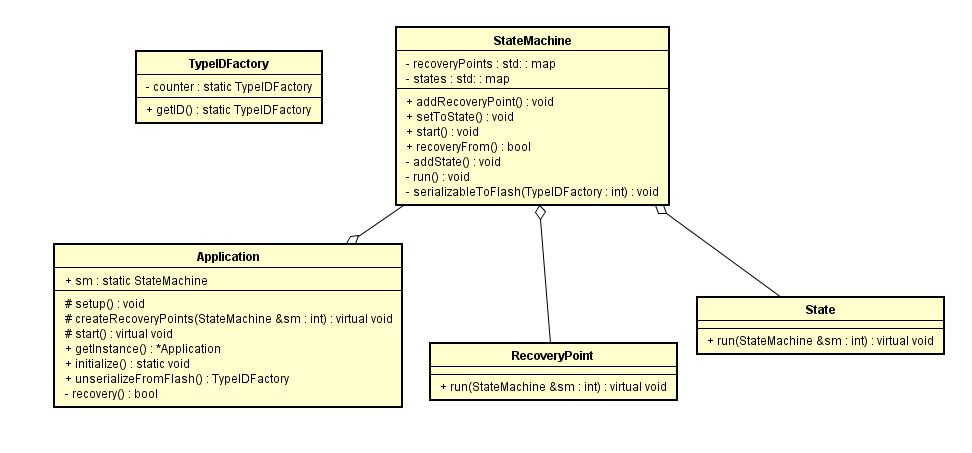
\includegraphics[width=0.9\textwidth]{figuras/diagramaFaultRecovery.jpg}
	\caption[Diagrama de classes da biblioteca \textit{FaultRecovery}.]{Diagrama de classes da biblioteca \textit{FaultRecovery}.}
	\label{Img:diagramaFaultRecovery}	
	%width=0.5\textwidth (Tamanho da Imagem)
\end{figure}

O uso do padrão de projeto mencionado e a aplicação dos conceitos de orientação a objetos possibilitou a criação de programas modularizáveis, em outras palavras, o código do \textit{firmware} pode ser separado por responsabilidades. Cada estado contém a sua classe de implementação, permitindo a separação do código e facilitando o entendimento da equipe. A primeira versão da biblioteca possuia três classes: \textit{TypeIDFactory, State} e \textit{StateMachine}, descritas abaixo:

\begin{itemize}
	\item \textit{\textbf{TypeIDFactory}} - Esta classe é responsável pela geração dos IDs de identificação dos estados. Os identificadores são únicos e auto-incrementais. Estes IDs são utilizados para indexar os estados em um \textit{hash map}.
	
	\item \textit{\textbf{State}} - Esta classe é responsável pela representação de um estado. Composta por um método abstrato \textit{run}, é a classe base para todos os estados do \textit{firmware}. No método \textit{run} o usuário implementa as rotinas de execução do estado. Caso ao final dessa rotina haja uma transição para um novo estado, o método \textit{setToState} deve ser invocado passando entre os sinais ($<$ $>$) a classe que representa o próximo estado a ser executado, conforme demonstrado no \autoref{Func:faultRecovery}. Apenas a classe é passada como parâmetro do \textit{template}, uma vez que a própria \textit{StateMachine} é responsável pela alocação dos objetos em seu \textit{hash map}. Essa abordagem evita cópias desnecessárias e perda de desempenho.
	
	\item \textit{\textbf{StateMachine}} - Esta classe representa a máquina de estados e tem a responsabilidade de controlar o despacho das funções implementadas em cada estado. Funciona como uma espécie de ``engrenagem'', que controla as transições entre os diversos estados do sistema, instanciando e adicionando os novos estados em um \textit{hashmap} e selecionando-os a cada transição do programa. A escolha de um \textit{hash map} deveu-se ao seu desempenho ser superior a outras estruturas de dados, uma vez que os estados são indexados pelos seus IDs.
	
	Conforme mostrado na Figura \ref{Img:fluxoFaultRecovery} no momento em que o programa recebe um evento responsável pela mudança de estado, o método \textit{setToState} desta classe recebe o valor da variável \textit{current} (determina o estado atual). Se o estado não estiver sido adicionado no \textit{map} de estados da máquina de estados, o método \textit{addState} será chamado para incluir esse novo estado.
	
	 Para executar a máquina de estados, deve-se instanciar um objeto \textit{StateMachine} e chamar o método \textit{start}, passando entre ($<$ $>$) o estado inicial conforme demonstrado no \autoref{Func:faultRecovery}, o método \textit{start} chamará o método \textit{setToState} e o método \textit{run}. Este Executará a máquina de estados por meio de um \textit{loop}. Aquele atribuirá o id do estado inicial para a variável \textit{current}.
		
\end{itemize}

\begin{figure}[H]
	\centering
	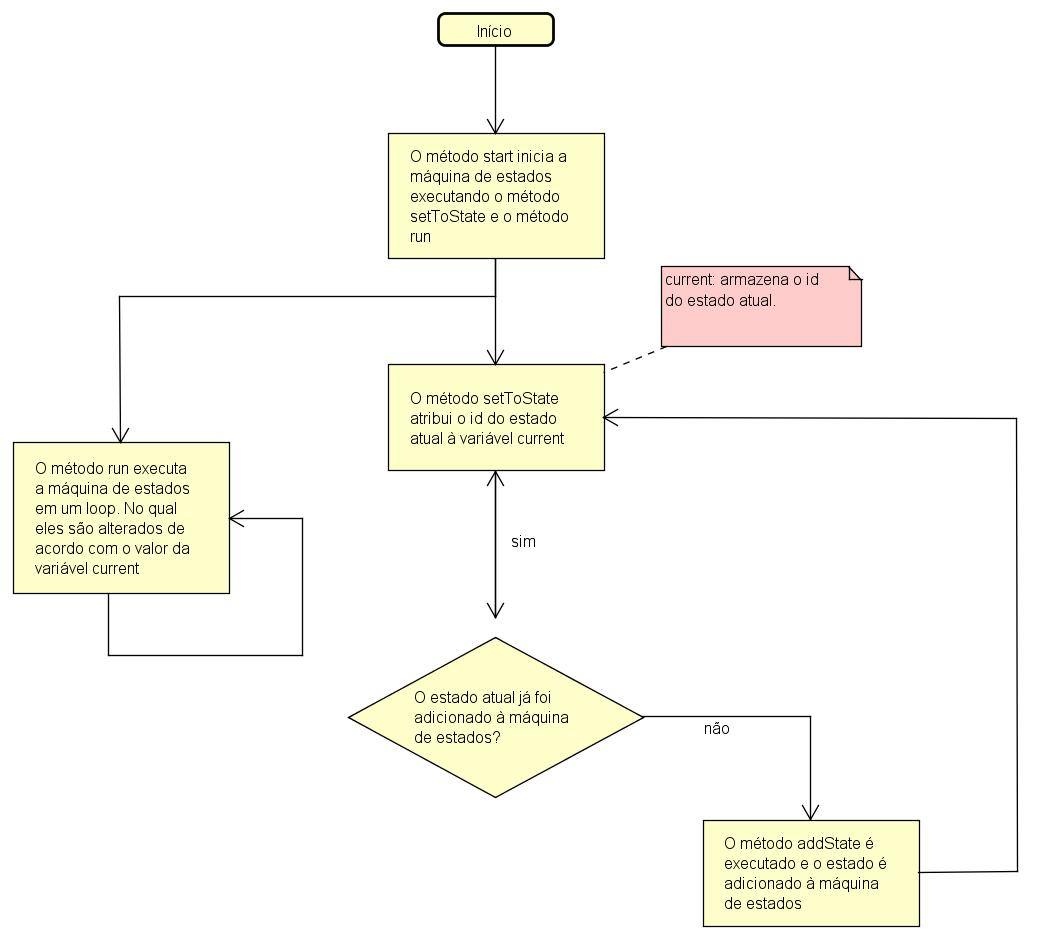
\includegraphics[width=0.9\textwidth]{figuras/fluxoFaultRecovery.jpg}
	\caption[Fluxograma da biblioteca \textit{FaultRecovery}.]{Fluxograma da biblioteca \textit{FaultRevorery}.}
	\label{Img:fluxoFaultRecovery}	
	%width=0.5\textwidth (Tamanho da Imagem)
\end{figure}
\newpage
\begin{lstlisting}[label=Func:faultRecovery,caption={[Exemplo de criação de um estado]A classe EsperandoCarroChegar herda da classe \textit{State} e tem sua rotina implementada no método \textit{run}, ao encerrar a rotina o método \textit{setToState} é invocado, alterando o estado atual. No método \textit{main} um objeto \textit{StateMachine} é instanciado e o método \textit{start} é chamado, iniciando a máquina de estados. Este quadro tem como objetivo demonstrar a utilização da biblioteca, apenas um estado será posto no quadro, os demais podem ser acessados no endereço \url{https://github.com/cleitonalmeida1}.}]
	class EsperandoCarroChegar: public State {
		void run(StateMachine &sm) {
			if (carroChegou()) {
				sm.setToState<EsperandoApertarBotao>();
			}
		}
	};
		int main() {
		StateMachine sm;
		sm.start<EsperandoCarroChegar>();
	}
\end{lstlisting}

Um exemplo simples para ilustrar a utilização da nova \textit{FaultRecovery} é o programa de estacionamento de um shopping. A entrada do estacionamento possui um emissor de \textit{tickets}, dois sensores e uma cancela. Ao se aproximar da cancela, o motorista aperta um botão para emitir um \textit{ticket}, após a emissão a cancela é aberta, os sensores detectam a entrada do carro ao interior do estacionamento e a cancela é fechada.

A máquina de estados do caso ilusório é composta por quatro estados, um deles é demonstrado no \autoref{Func:faultRecovery}:

\begin{itemize}
	\item \textbf{EsperandoCarroChegar} - Este é o estado inicial da máquina de estados. O sensor de presença detecta a chegada do veículo na entrada do estacionamento, o carro se aproxima da entrada, então o estado EsperandoCarroChegar detecta a aproximação do veículo e chama o próximo estado.
	
	\item \textbf{EsperandoApertarBotao} - Neste estado o dispositivo eletrônico emite o \textit{ticket} de estacionamento após o motorista apertar o botão. Após isso, o estado atual é alterado para EsperandoCarroEntrar. Outra situação é quando o motorista decide não adentrar ao estacionamento, neste caso o estado é alterado para o anterior (EsperandoCarroChegar). 
	
	\item \textbf{EsperandoCarroEntrar} - Neste estado os sensores estão aguardando a entrada do carro ao estacionamento. O sensor externo ao estacionamento detecta duas situações, a primeira é quando o carro se afasta da cancela e não entra no estacionamento, neste caso a máquina de estados retorna ao seu estado inicial. O segundo é quando o carro adentra ao estacionamento, neste caso o sensor externo identifica a entrada do carro, o interno ao estacionamento detecta o carro se afastando da cancela, com o seu afastamento o sistema altera o estado para FecharCancela.
	
	\item \textbf{FecharCancela} - Neste estado o carro se afasta da entrada do estacionamento, o sensor externo a esse detecta o afastamento do carro e a cancela é fechada. Ao fechar a cancela o estado FecharCancela, por ser o último estado da máquina de estados, irá chamar o estado inicial, para então reiniciar o ciclo de execução dos estados.
	
\end{itemize}


\subsection{Refatoração e Aperfeiçoamento: Versão 2.0} \label{subsec:versao2}

Na Subseção \ref{subsec:versao1} que trata da versão 1.0 da biblioteca, mostrou-se como implementar os estados de uma máquina de estados. Esta subseção trata da criação dos pontos de recuperação, como inicializar a máquina de estados e quais as classes adicionadas na biblioteca e suas responsabilidades. Nesta etapa de desenvolvimento, focou-se na tolerância a falhas. A versão 2.0 da biblioteca \textit{FaultRecovery} utiliza a máquina de estados desenvolvida na versão 1.0, no entanto foi adicionada a funcionalidade que possibilita a criação de pontos de recuperação de falhas. Se o microcontrolador trava durante a execução da máquina de estados, o defeito é detectado pelo \textit{whatchdog}, já que o temporizador tem seu valor de limiar excedido, e então o \textit{whatchdog} reinicia o dispositivo. Ao restaurar, é possível diagnosticar o último estado seguro, pois esta informação foi gravada na \textit{flash} durante as trocas de estado. Caso exista algum ponto de recuperação configurado para este último estado seguro, será executado. 

O usuário da biblioteca deve criar os pontos de recuperação conforme seja necessário, sendo possível adicionar no máximo um ponto de recuperação por estado. Estes pontos indicam quais as rotinas deverão ser executadas caso o programa falhe durante a execução do estado especificado. Essa rotina pode executar uma determinada configuração no microcontrolador ou uma tarefa que deva ser iniciada antes da máquina de estados ser inicializada.

As classes \textit{Application} e \textit{RecoveryPoint} foram adicionadas à biblioteca. A primeira é responsável pela inicialização do \textit{firmware} e gerenciamento dos pontos de recuperação, a segunda é responsável pela implementação dos pontos de recuperação. Para utilizar a versão 2.0, deve-se instanciar um objeto \textit{Application} e chamar o método \textit{initialize} da seguinte forma: Application:initialize$<$EstacionamentoApp$>$. A classe EstacionamentoApp é herdada de \textit{Application}, que possibilita a implementação de três métodos, sendo o método \textit{start} obrigatório (pois é puramente virtual) e os métodos \textit{creatRecoveryPoints} e \textit{setup} opcionais (pois não são puramente virtuais). O método \textit{initialize} é \textit{static}, ou seja, ele pode ser chamado a partir de um código externo à classe sem a necessidade de criar uma nova instância de \textit{Application}. Ao evocar o método \textit{initialize}, um objeto \textit{StateMachine} é inicializado, uma instância da classe EstacionamentoApp também é inicializada, essa será utilizada durante toda a execução da máquina de estados. Após o EstacionamentoApp ser inicializado, quatro métodos serão evocados automaticamente. 

O primeiro é o método \textit{setup} que poderá ou não ser implementado. Neste método são implementadas as configurações do microcontrolador, que podem variar dependendo do seu modelo, vale ressaltar que a utilização desta biblioteca não se limita ao microcontrolador \textit{mbed}, pois os extensionistas do projeto Coxim Robótica do Campus de Coxim - UFMS já estão utilizando a arquitetura da biblioteca \textit{FaultRecovery} adaptada para a plataforma \textit{arduino}, por exemplo, no método \textit{setup} os extensionistas programaram as configurações iniciais de um robô seguidor de linha e cada aluno ficou responsável por implementar um estado da máquina de estados do carrinho.

O segundo é o método \textit{createRecoveryPoints}, que poderá ou não ser implementado, pois por padrão esse método não adiciona nenhum ponto de recuperação à máquina de estados. Entretanto pode ser sobrescrito, caso necessário, para que pontos de recuperação sejam adicionados à máquina de estados. Para implementar um ponto de recuperação deve-se criar uma classe que herde de \textit{RecoveryPoints}. 

Ao herdar dessa classe, o usuário obrigatoriamente deverá implementar o método abstrato \textit{run} no qual conterá as rotinas de execução caso o programa seja restaurado daquele ponto. Para adicionar um ponto de recuperação à máquina de estados, deve-se utilizar o método \textit{addRecoveryPoint} nativo da classe \textit{StateMachine} e evocá-lo conforme demonstrado no quadro \autoref{Func:addRecoveryPoint}. Esse receberá entre $< >$ o ponto de recuperação e o estado ao qual ele pertence, sendo assim o ponto de recuperação fica associado ao estado, em outras palavras, o id de identificação do estado no \textit{hashmap} de estados será o mesmo do seu ponto de recuperação no \textit{hashmap} de pontos de recuperação.

Como mencionado, na versão 2.0 o método \textit{setToState} da classe \textit{StateMachine} além de trocar o estado atual, também armazena o seu id na memória flash do microcontrolador \textit{mbed}. Quando o dispositivo for reiniciado, se existir um ponto de recuperação para o id armazenado na memória \textit{flash} a biblioteca executará o ponto de recuperação referente ao id lido da memória \textit{flash}.

O terceiro é o método \textit{start} no qual é realizada a inicialização da máquina de estados conforme demonstrada no segundo parágrafo desta Subseção.

\begin{lstlisting}[label=Func:addRecoveryPoint,caption={[Métodos \textit{createRecoveryPoints} e \textit{run}]Este quadro demonstra a implementação do método \textit{createRecoveryPoints} implementado no EstacionamentoApp que herda de \textit{Application}. O ponto de recuperação é criado quando o método \textit{addRecoveryPoint} é evocado, percebe-se que existem duas classes separadas por vírgula e entre $<$$>$, a primeira é a implementação do ponto de recuperação, ou seja, a classe que herda de \textit{RecoveryPoints}. A segunda é a classe que representa o estado que deverá ser executado após a reinicialização do microcontrolador, ou seja, caso ele inicie neste ponto de recuperação o estado EsperandoCarroEntrar deverá ser escutado. No método \textit{run} da classe RecoveryEsperandoCarroEntrar encontra-se o código que será executado caso o microncontrolador falhe no momento em que o carro iria entrar no estacionamento. Se a energia acabasse durante o fechamento da cancela e o programa tivesse voltado com a cancela aberta, o dono do estacionamento teria prejuízo, pois alguns carros poderiam entrar sem pagar a taxa de estacionamento enquanto a cancela estivesse aberta.}]
	//Estacionamento App Class
	void EstacionamentoApp::createRecoveryPoints(StateMachine &sm) {
		sm.addRecoveryPoint<RecoveryFecharCancela, FecharCancela>();
	}

	//RecoveryFecharCancela Class
	void RecoveryFecharCancela::run(StateMachine &sm) {
		if (checarPortaoAberto()) {
			fecharPortao();
		}
		sm.start<EsperandoCarroEntrar>();
	}
\end{lstlisting}

\newpage

\section{\textit{Classe de Redundância de Dados: TData}} \label{sec:classeTData}

A classe \textit{TData} foi implementada com o objetivo de obter-se uma redundância de dados automatizada, tanto para variáreis primitivas (int, float, long, double, char, bool), quanto para objetos de uma classe. Existem duas maneiras de se criar um objeto \textit{TData}, a primeira é utilizando tipos primitivos e a segunda objetos. 

Ao instanciar um objeto \textit{TData}, deve-se especificar o seu tipo e passar um valor ou um objeto no construtor: TData$<$tipo\_da\_variável$>$ variavel(valor). Ou o valor, ou o objeto passado como parâmetro serão copiados para três cópias de segurança, das quais serão utilizadas para manter a integridade do valor original por meio de um sistema de votação, que verifica se os valores das cópias são consistentes.

\subsection{Classe TData com Tipos Primitivos} \label{subsec:TDataPrimitivo}

O método \textit{setData} (pertencente a classe \textit{TData}) será invocado automaticamente ao passar o número inteiro 4 como parâmetro no construtor da classe. Ao alterar o valor 4 para a operação 1 + 9, o método \textit{setData} será implicitamente chamado por meio de sobrescrita de operadores, disponível na linguagem C++, possibilitando que o valor da variável seja atualizado juntamente com as cópias de segurança. Vale ressaltar que a cada vez que o objeto \textit{TData} for acessado, o método \textit{getByVotting()} que implementa um esquema de votação será executado, validando todas as cópias do objeto \textit{TData}. A injeção de falhas foi realizada por meio do método temporário chamado \textit{injectFault}, que modificou o valor de uma das cópias do objeto \textit{TData}, simulando o fenômeno \textit{bit-flip}. Esse método foi utilizado durante a implementação da classe \textit{TData}, sendo retirado dela após sua conclusão. Na Figura \ref{Img:tdataPrimitivo} é mostrado os valores das cópias após a injeção de falhas.

\begin{figure}[H]
	\centering
	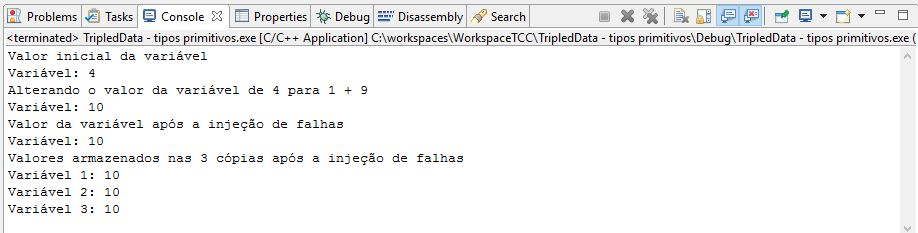
\includegraphics[width=1.0\textwidth]{figuras/tdataPrimitivo.jpg}
	\caption[Figura que apresenta a saída com os valores das cópias consistentes para tipos primitivos após a injeção de falhas.]{Nesta figura é mostrado que o valor das cópias foram atualizados após a operação 1 + 9. Também é mostrado que os valores das cópias continuaram consistentes após a injeção de falhas.}
	\label{Img:tdataPrimitivo}	
	%width=0.5\textwidth (Tamanho da Imagem)
\end{figure}	


\subsection{Um Exemplo Ilusório Para Utilização da Classe TData com Objetos} \label{subsec:exemploTData}

Para demonstrar como utilizar e instanciar a classe \textit{TData} com objetos, foi utilizado um exemplo que permitiu a utilização de objetos heterogêneos, ou seja, objetos que possuem outros objetos dentro de si, que podem ser objetos de pilha ou ponteiros para um endereço de memória. Destaca-se, um caso ilusório de um automóvel inteligente interligado a diferentes tipos de dispositivos e formas de comunicação, comunicando-se a um servidor. 

As informações disponibilizadas pelo veículo são navegação, diagnósticos do funcionamento do próprio veículo, dentre outras informações. Este por sua vez sofre um acidente e o sistema se encarrega de acionar outro sistema, ou seja, o sistema embarcado instalado no carro se comunica com outro remotamente. Este, por sua vez, receberia todos os dados relativos ao paciente, inclusive sua localização para um possível deslocamento de ambulâncias \cite{Valderi:2008}. Este exemplo foi implementado de maneira simples com o objetivo de demonstrar como instanciar e utilizar a classe \textit{TData}. 

Foram criadas duas classes para compor o cenário, sendo elas as classes Carro e Emergência, essas classes tiveram seus operadores de igualdade implementados pois, a classe \textit{TData} obriga que suas implementações sejam realizadas, visto que o compilador não é capaz de definir o comportamento de uma definição de igualdade em um objeto. Cada objeto define a igualdade de um jeito diferente, a classe \textit{string} por exemplo, define que igualdade são objetos com o mesmo conteúdo, ainda que sejam objetos distintos, ou seja, em endereços de memória diferentes.

A implementação dos operadores de igualdade para tipos primitivos não é obrigatória pois são tipos homogêneos, já os objetos podem ter outros objetos em seu escopo, como é o exemplo da classe Carro, que contém uma instância da classe Emergência em seu escopo, tornando obrigatória a implementação de seus operadores de igualdade, para que possam ser utilizados na classe \textit{TData}.

\subsection{Classe Carro com Objeto de Pilha} \label{subsec:classeObjetoPilha}

Para instanciar um objeto \textit{TData} do tipo Carro, primeiro deve-se declarar um objeto carro e setar os valores de seus atributos e consecutivamente instanciar um objeto \textit{TData} do tipo carro passando o objeto carro recém criado como parâmetro no construtor da classe com os seus valores preenchidos. 

Para este exemplo utilizou-se as classes Carro e Emergencia mencionadas nas Seções anteriores e o método \textit{injectFault} utilizado para simular o fenômeno \textit{bit-flip}. A injeção de falhas foi realizada com métodos temporários implementados dentro da classe \textit{TData} alterando os valores do telefone do hospital pertencente a classe Emergencia e da localização do carro pertencente a classe Carro.

O carro possui um sistema inteligente interligado com outros sistemas, ao sofrer o acidente automaticamente o sistema embarcado instalado no carro iria se conectar a outro sistema pedindo socorro e enviando sua localização para o hospital, essa por sua vez poderia ser alterada por alguma falha em seu endereço de memória podendo causar a morte do motorista, pois a ambulância seria enviada para outro endereço que não fosse o do carro. Após a injeção de falhas, os valores  de todas as cópias podem ser visualizados na Figura \ref{Img:tdataObjetoPilha} demonstrando que mesmo após a ocorrência de falhas nos endereços de memória da localização e do telefone do hospital, as cópias continuaram consistentes.

\begin{figure}[H]
	\centering
	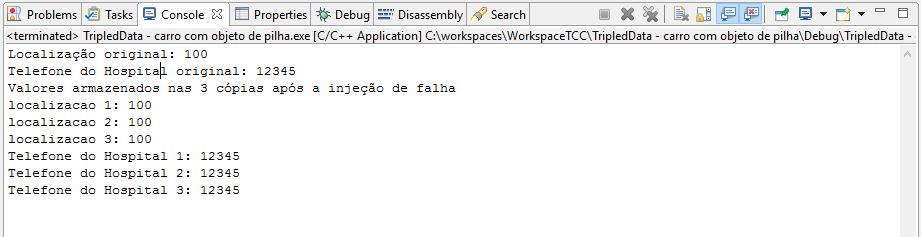
\includegraphics[width=1.0\textwidth]{figuras/tdataObjetoPilha.jpg}
	\caption[Valores das cópias consistentes após a injeção de falhas com objeto de pilha.]{Nesta figura é mostrado que valores das cópias continuaram consistentes após a injeção de falhas.}
	\label{Img:tdataObjetoPilha}	
	%width=0.5\textwidth (Tamanho da Imagem)
\end{figure}

\subsection{Classe Carro com Ponteiro} \label{subsec:CarroPonteiro}

Este parágrafo tem por objetivo demonstrar que a classe \textit{TData} também funciona com ponteiros. A classe \textit{TData} também pode receber como parâmetro em seu construtor objetos que contenham referência para endereços de memória. Realizou-se uma injeção de falhas no ponteiro emergencia (armazena o telefone do hospital), alterando o seu endereço de memória por meio do método \textit{injectFault}. Os valores do telefone e da localização após a injeção de falhas é mostrado na Figura \ref{Img:tdataPonteiro}, mostrando que mesmo após a modificação do endereço de memória do ponteiro emergência em uma das cópias, o valor do telefone do hospital continua o mesmo para todas as cópias.

\begin{figure}[H]
	\centering
	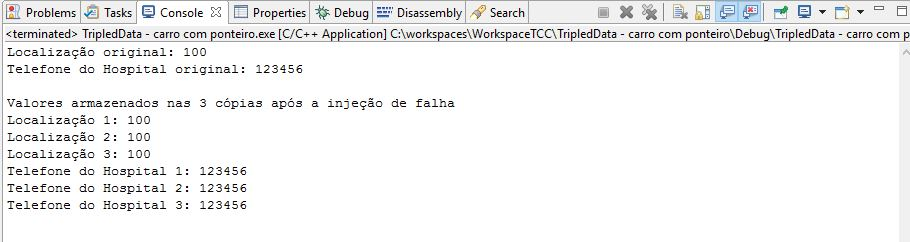
\includegraphics[width=1.0\textwidth]{figuras/tdataPonteiro.jpg}
	\caption[Valores das cópias consistentes após a injeção de falhas com ponteiro.]{Nesta figura é mostrado que os valores das cópias continuaram consistentes após a injeção de falhas.}
	\label{Img:tdataPonteiro}	
	%width=0.5\textwidth (Tamanho da Imagem)
\end{figure}

Além das três cópias de segurança que compõem a classe \textit{TData} existe mais uma cópia chamada \textit{dataObject}, utilizada para atualizar o objeto \textit{TData} sem a necessidade de passar o objeto modificado como parâmetro no construtor da classe. A variável \textit{dataObjet} é utilizada para replicar uma alteração no objeto para as demais cópias. Para acessar o objeto \textit{dataObject} é necessário chamar o método \textit{getDataObject} implementado para atualizar as três cópias e executar o método \textit{getByVotting} para manter a consistência de todas as cópias. Na Figura \ref{Img:tdataSetando} é mostrada a atualização do telefone do hospital e os valores das cópias após a injeção de falhas.

\begin{figure}[H]
	\centering
	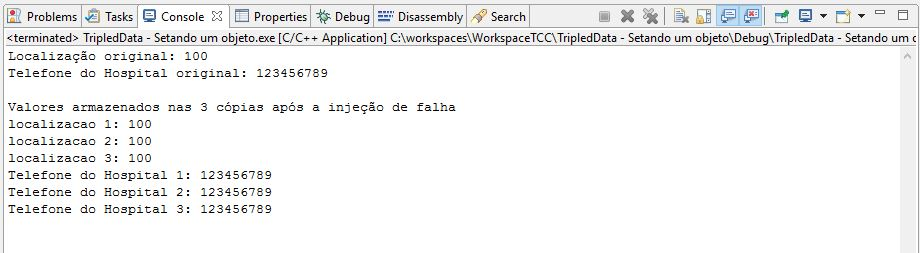
\includegraphics[width=1.0\textwidth]{figuras/tdataSetando.jpg}
	\caption[Figura que apresenta a saída com os valores das cópias consistentes após a atualização do objeto \textit{TData} do tipo carro e da injeção de falhas.]{Figura que apresenta a saída com os valores das cópias consistentes após a atualização do objeto \textit{TData} do tipo carro e da injeção de falhas.}
	\label{Img:tdataSetando}	
	%width=0.5\textwidth (Tamanho da Imagem)
\end{figure} % Aplicação
	%====================================================================================================
%----------------------------------------------------------------------------------------------------
% Autor				: Vagner da Silva Bezerra
%----------------------------------------------------------------------------------------------------
% Data de criação	: 10 de Outubro de 2016
%====================================================================================================

\chapter{Resultados} \label{cap:Resultados}

Neste capítulo são apresentados os resultados dos testes realizados. 

\section{Desempenho da Biblioteca \textit{FaultRecovery}} \label{Sec:tempoRecovery}

Esta Seção tem como objetivo demonstrar o desempenho da biblioteca \textit{FaultRecovery} em termos de tempo de execução. Para realizar os testes, utilizou-se cinco algoritmos de ordenação \textit{bubble sort, insertion sort, merge sort} e \textit{comb sort} \cite{orderUnicamp, vivaLinux}, a execução dos cinco algoritmos forma um ciclo de teste. Ao todo cada ciclo foi executado cem vezes. Os algoritmos foram implementados para ordenar os elementos em forma crescente em um microcontrolador \textit{mbed} LPC1768. Para cada ciclo de teste, utilizou-se um vetor do tipo \textit{unsigned short} contendo 4096 elementos enumerados em ordem decrescente de $n$ (4096) até 1, ou seja, o elemento da primeira posição recebeu o valor $n$, o da segunda $n-1$, e assim sucessivamente até o elemento da última posição receber o valor 1. Essa estratégia foi utilizada para que o tempo de execução dos algoritmos fosse similar, pois se o vetor estivesse com números aleatórios ao invés de decrescente, isso poderia afetar o comportamento dos algoritmos. Por isso tentou-se manter um padrão para que fosse possível medir o tempo da biblioteca. O tamanho total do vetor totalizou 8kB de memória (2 bytes * 4096). Tentou-se aumentar a quantidade de elementos do vetor, entretanto quando se tentou alocar um espaço de memória maior que 8kB, o \textit{firmware} teve sua execução interrompida no primeiro ciclo de teste, em outros no segundo.

O primeiro teste teve como objetivo medir o tempo de execução dos algoritmos de ordenação, simulando um \textit{firmware} implementado por um usuário que não utilizou a biblioteca \textit{FaultRecovery}. Todos os algoritmos compartilharam do mesmo vetor, por isso, antes de cada ordenação foi necessário desordenar o vetor para cronometrar o tempo real de ordenação. O tempo de cada algoritmo foi cronometrado, desde o início de sua execução até seu fim, sendo desprezado o tempo de desordenação do vetor.

O segundo teste teve como objetivo medir o tempo de execução dos mesmos algoritmos de ordenação, fazendo uso da biblioteca \textit{FaultRecovery}. O tempo de execução no segundo teste foi medido a partir do início da execução de um estado da máquina de estados até o fim dele. Tanto para o primeiro quanto para o segundo teste foi utilizada a mesma quantidade de elementos do vetor (4096), a mesma sequência de execução (\textit{bubble, insertion, selection, merge} \textit{e comb}) e o tempo de desordenação do vetor também foi desprezado. Ao final das cem execuções do primeiro e do segundo teste, as médias de tempo de execução para cada algoritmo e para cada ciclo de teste foram calculadas. O tempo de execução da biblioteca \textit{FaultRecovery} também foi calculado, obtendo-se o resultado mostrado na Figura \ref{Img:tempoRecovery}.

\begin{figure}[h]
	\centering
	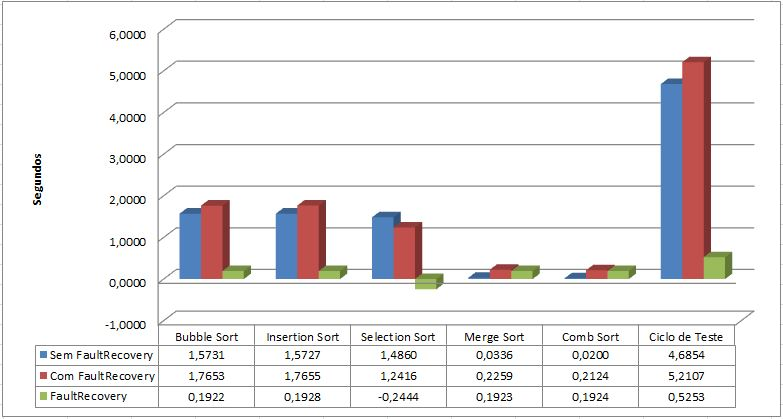
\includegraphics[width=0.9\textwidth]{figuras/tempoRecovery.jpg}
	\caption[Tempo de execução da biblioteca \textit{FaultRecovery}]{Nesta Figura são mostrados os resultado dos testes de medição do tempo de execução dos algoritmos de ordenação, sem a biblioteca e com a biblioteca. Percebe-se que com a utilização da biblioteca o tempo de execução dos algoritmos aumentou em média 0,5253 segundos ou 525,3 milisegundos.}
	\label{Img:tempoRecovery}	
	%width=0.5\textwidth (Tamanho da Imagem)
\end{figure}	
\newpage
Dentre os tempos de execução mostrados na Figura \ref{Img:tempoRecovery}, obteve-se um resultado inesperado: o tempo de execução do algoritmo \textit{insertion sort} foi menor com a biblioteca \textit{FaultRecovery}, mesmo ela gerando um maior tempo de execução (devido à gerência da estrutura de sua máquina de estados). Diante disso, verificou-se a implementação dos dois testes, e não foi constatada nenhuma diferença entre os códigos que pudessem causar este resultado. Então, um terceiro teste foi executado outras cem vezes, utilizando-se um vetor de 6KB (menor que o utilizado nos testes anteriores) para verificar se o comportamento anômalo persistiria em ocorrer. O resultado foi similar, ou seja, o comportamento persistiu, mas como não havia tempo hábil para uma análise aprofundada, presumiu-se que esses casos são factíveis de ocorrer, provavelmente devido as otimizações de código feitas pelo compilador, já que o microcontrolador utilizado nos testes não possui sistema operacional e nenhuma outra aplicação rodando simultaneamente. Portanto verificou-se que quanto maior o volume de dados do vetor, o tempo de execução da \textit{FaultRecovery} torna-se menos expressivo. Os resultados do terceiro teste são mostrados na Figura \ref{Img:tempoRecovery2}.

\begin{figure}[h]
	\centering
	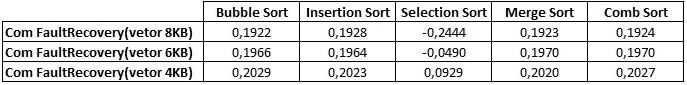
\includegraphics[width=0.9\textwidth]{figuras/tempoRecovery2.jpg}
	\caption[Tempo de execução da biblioteca \textit{FaultRecovery} com três tamanhos de vetores diferentes.]{Nesta Figura é mostrado o tempo de execução da biblioteca \textit{FaultRecovery} com três vetores de tamanhos diferentes. Percebe-se que o tempo de execução da biblioteca no algoritmo \textit{insertion sort} é negativo no primeiro e no segundo teste, contudo no teste com o vetor de tamanho 4KB obteu-se um tempo de execução positivo. Portanto verificou-se que quanto maior o volume de dados do vetor, o tempo de execução da \textit{FaultRecovery} torna-se menos expressivo.}
	\label{Img:tempoRecovery2}	
	%width=0.5\textwidth (Tamanho da Imagem)
\end{figure}
\newpage
\section{Desempenho e Eficiência da Classe TData} \label{Sec:tempoTData}

Para testar a eficácia e o desempenho da classe \textit{TData} foram realizados dois tipos de testes. O primeiro não utilizou a classe \textit{TData} e o segundo a utilizou. Em ambos o vetor foi preenchido de forma decrescente e foram realizados cem ciclos de execuções, conforme descrito no primeiro parágrafo da Seção \ref{Sec:tempoRecovery}. No entanto houve a necessidade de reduzir o tamanho do vetor de 4096 para 1024 elementos, devido à redundância de dados da classe \textit{TData}, pois ela copia um valor para três endereços de memória diferentes. Se fossem utilizados os 4096 elementos, a quantidade de memória alocada seria de aproximadamente 32kB, pois cada elemento que antes ocupava 2 bytes, passaria  utilizar 8 bytes. Isso impossibilitaria a realização dos testes. 


O primeiro teste, que não utilizou a classe \textit{TData}, teve como objetivo medir o tempo de execução de cada algoritmo de ordenação. Nele, a biblioteca \textit{FaultRecovery} não foi utilizada, foi levado em conta apenas o tempo de execução de cada algoritmo. O resultado do primeiro teste foi comparado ao do segundo, obtendo-se o tempo de execução conforme mostrado na Figura \ref{Img:tempoTData}. Para iniciar o segundo teste, foi necessário apenas substituir a declaração do vetor de \textit{unsigned short vetor[n]} para \textit{TData$<$unsigned short$>$ vetor[$n$]}, isso mostra que a \textit{TData} aplica redundância de dados de forma simples, reduzindo a reescrita de várias linhas de código.

Foram determinados três parâmetros de teste para deliberar se um ciclo de teste falhou ou não. Como o vetor possuía 1024 elementos ordenados em ordem decrescente de $n$ até 1, o resultado de uma ordenação crescente é conhecido. Após a injeção de falhas no microcontrolador \textit{mbed}, alterando um endereço de memória aleatório, estabeleceu-se que para um ciclo de teste falhar ele deveria ter entre 10\%, 25\% ou 50\% dos 1024 elementos diferentes do resultado conhecido. Essa estratégia foi utilizada para se ter uma medida reduzida (10\%), média (25\%) e extrema (50\%) de falhas.

Conforme exibido na Figura \ref{Img:falhaTData}, o teste sem a \textit{TData} para a quantidade de falhas acima de 10\% foi de 20\% para cada ciclo de testes. Com a \textit{TData} esse número caiu para zero. Em contrapartida, notou-se uma diferença média de 0,2658 segundos a mais no tempo do ciclo com redundância de dados. 

%[UMA DÚVIDA: NA SEÇÃO ANTERIOR, OS ELEMENTOS DO VETOR TAMBÉM ERAM DISPOSTOS DE 1 A N DE FORMA DECRESCENTE? SE SIM, POR QUE NÃO FOI MENCIONADO?]

%Para testar a eficácia e o desempenho da classe TData foram realizados dois tipos de testes. Em ambos, os elementos do vetor foram enumerados decrescentemente de 1 até $n$. A primeira posição recebeu o valor $n$, a segunda $n-1$, e assim sucessivamente até a última receber o valor 1. Assim como os testes mencionados na Seção \ref{Sec:tempoRecovery}, nestes também foram realizados cem ciclos de execução, no entanto houve a necessidade de reduzir o tamanho do vetor de 4096 para 1024 elementos, devido à redundância de dados da classe TData, pois ela copia um valor para três endereços de memória diferentes. Se fossem utilizados os 4096 elementos a quantidade de memória alocada seria de aproximadamente 16KB, impossibilitando a realização dos testes. [POR QUE NAO PODERIA COM 16KB?] 

%O primeiro não utilizou a classe TData e o segundo a utilizou. O teste que não utilizou a classe TData teve como objetivo medir o tempo de execução de cada algoritmo de ordenação. Nele, a biblioteca \textit{FaultRecovery} também não foi utilizada [E NO SEGUNDO, FOI? PORQUE SE NÃO FOI, VOCÊ PODE FALAR QUE NÃO UTILIZOU DE FORMA GERAL], foram levados em conta apenas o tempo de execução de cada algoritmo. O resultado do primeiro teste foi comparado ao do segundo, obtendo-se o tempo de execução da classe TData conforme demonstrado na Figura \ref{Img:tempoTData}. Para iniciar o segundo teste, apenas foi necessário substituir a declaração do vetor de \textit{unsigned short vetor[n]} para \textit{TData$<$unsigned short$>$ vetor[$n$]}, isso mostra que a TData permite redundância de dados sem a reescrita de muitas linhas de código.

%Notou-se uma diferença média de 0,2658 segundos do tempo de execução de um algoritmo de ordenação sem redundância de dados para um com redundância de dados. No entanto, deve-se levar em conta que o teste realizado sem a classe TData falhou em vários [FORAM VÁRIOS OU FORAM TODOS?] ciclos de teste, conforme mostra-se na Figura \ref{Img:falhaTData}, que exibe os resultados do primeiro e do segundo teste. 

%Foram determinados três parâmetros de teste para determinar se um ciclo de teste falhou ou não. Como o vetor possui 1024 elementos e o resultado de uma ordenação que inicia em 1 até 1024 é conhecida, após a injeção de falhas no microcontrolador \textit{mbed}, alterando um endereço de memória aleatório, estabeleceu-se que para um ciclo de teste falhar ele deve ter 10\%, 25\% ou 50\% dos 1024 elementos diferentes do resultado conhecido. 

Para os resultados acima de 10\%, 25\% e 50\% analisou-se os algoritmos de ordenação isoladamente e também cada ciclo de teste, lembrando que cada ciclo é representado pela execução dos cinco algoritmos de ordenação. Obteve-se os seguintes resultados, para os valores acima de 10\%, 25\% e 50\% de falhas respectivamente, 44\%, 25\% e 20\% dos ciclos de testes falharam. Percebe-se que o primeiro teste não possui redundância de dados, embora os cem ciclos de testes tenham sido executados, pode-se notar que os valores do vetor não continuaram os mesmos após a injeção de falhas. No entanto na Figura \ref{Img:falhaTData} é possível visualizar que mesmo após as injeções de falhas, a classe \textit{TData} se mostrou eficaz garantindo a consistência dos dados do vetor até o fim dos cem ciclos de teste.


\begin{figure}[h]
	\centering
	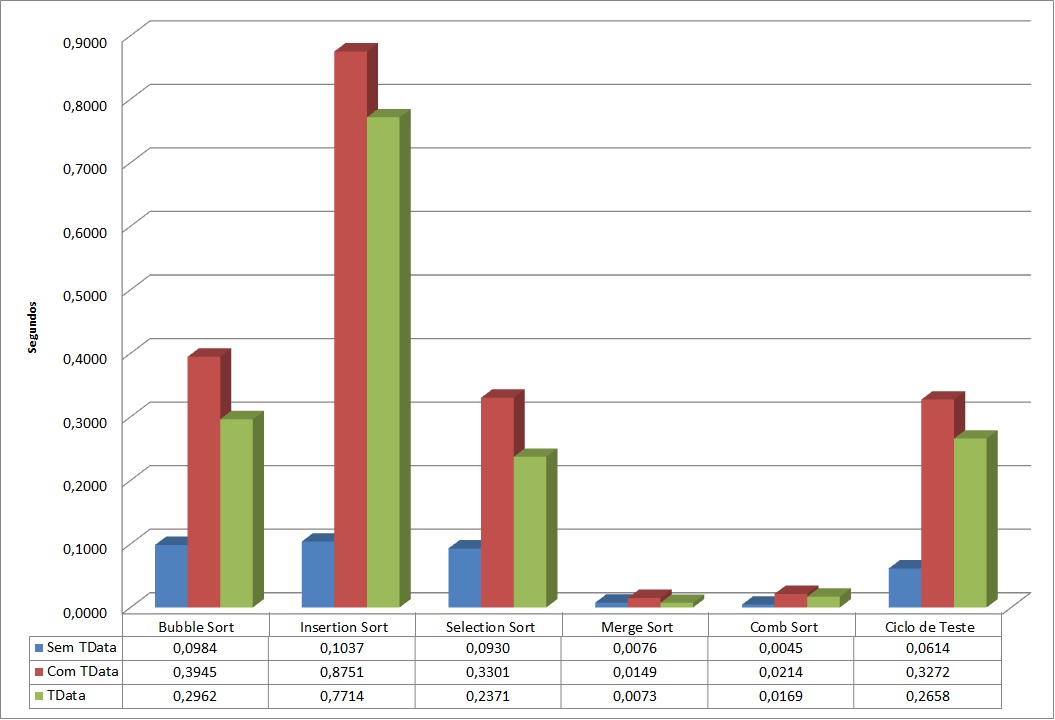
\includegraphics[width=0.9\textwidth]{figuras/tempoTData.jpg}
	\caption[Tempo de execução da Classe \textit{TData}]{O tempo de execução dos algoritmos sem a classe \textit{TData} foi relativamente baixo, sendo que o maior tempo atingiu 0,1037 segundos ou 103,7 milisegundos para ordenar um vetor de 1024 elementos. Já o tempo dos algoritmos com a Classe \textit{TData} foi um pouco maior, sendo o tempo de execução do algoritmo insertion sort que atingiu 0,8751 segundos ou 875,1 milisegundos. O tempo de execução médio da classe \textit{TData} para cada algoritmo de ordenação foi de 0,2658 segundos ou 265,8 milisegundos.}

	\label{Img:tempoTData}	
	%width=0.5\textwidth (Tamanho da Imagem)
\end{figure}

\begin{figure}[h]
	\centering
	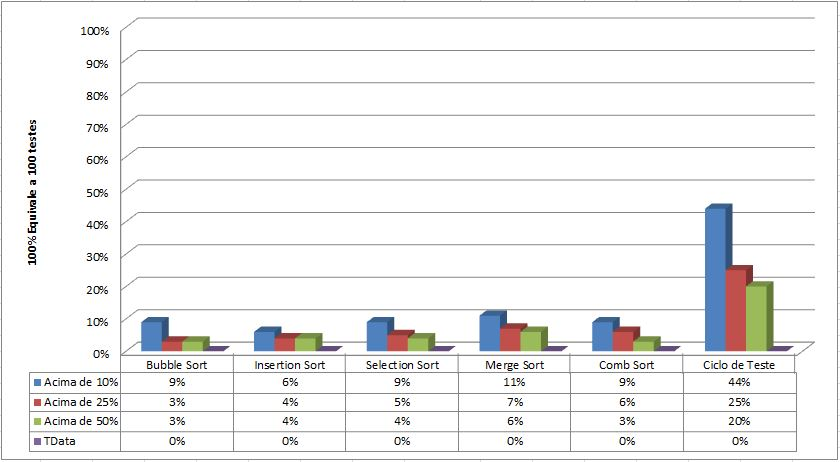
\includegraphics[width=0.9\textwidth]{figuras/falhaTData.jpg}
	\caption[Teste de redundância de dados da classe \textit{TData}]{Nesta Figura, para as falhas detectadas acima de 10\%, 25\% e 50\% são do teste que não utiliza redundância de dados, por exemplo, para as falhas acima de 10\%, aproximadamento 44\% dos ciclos de testes falharam. No entanto para o teste que utilizou a redundância de dados, nenhum algoritmo de ordenação ou ciclo de teste falharam. Embora o teste estivesse sendo bombardeado por falhas, a classe TData se mostrou eficaz corrigindo os valores alterados nos endereços de memória cobertos pela redundância de dados.}
	\label{Img:falhaTData}	
	%width=0.5\textwidth (Tamanho da Imagem)
\end{figure}

\newpage
\section{Recuperação de falhas da biblioteca \textit{FaultRecovery}}\label{Sec:recupeFault}

Nesta Seção são mostrados os resultados dos testes realizados com a biblioteca \textit{FaultRecovery}. O código utilizado na Seção \ref{Sec:tempoRecovery} foi modificado para injetar falhas em endereços de memória aleatórios. Foram utilizados os mesmos algoritmos de ordenação, no entanto o tempo de execução da biblioteca foi desprezado, pois o resultado avaliado neste teste foi a capacidade de recuperação de falhas. Se as falhas registradas nos resultados ocorressem em uma situação real, os dados afetados por essas falhas poderiam ocasionar o travamento do \textit{firmware}. Caso utilizado o mecanismo de \textit{watchdog} para a detecção de falhas, quando o \textit{whatchdog} percebesse que o microcontrolador estivesse travado, o \textit{mbed} seria reinicializado. No entanto, considerando-se o exemplo de uma estação meteorológica, se o travamento ocorresse no momento em que os dados coletados fossem enviados para um servidor remoto, por ser uma máquina de estados, no qual a ordem de execução de cada estado implica nos resultados obtidos, quando o \textit{mbed} fosse reinicializado, o primeiro estado que seria executado, poderia ou não ser o estado responsável que enviaria os dados ao servidor remoto.

Para que isso não venha a ocorrer, a estação meteorológica poderia ser implementada utilizando a biblioteca \textit{FaultRecovery} para que pontos de recuperação de falhas pudessem ser criados, para assim que o microcontrolador reinicializasse por conta de alguma falha, algum ponto de recuperação predefinido pudesse ser executado. Entretanto utilizou-se algoritmos de ordenação para simular uma máquina de estados. Foram criados pontos de recuperação para cada algoritmo de ordenação, se em algum momento o microcontrolador vier a travar e posteriormente ser reiniciado, seja manualmente ou automaticamente, o ponto de recuperação predefinido será executado. Mostra-se na Figura \ref{Img:testeFaultRecovery} os resultados obtidos após a execução de cem ciclos de testes, cada ciclo é representado pela execução dos cinco algoritmos de ordenação conforme descrito na Seção \ref{Sec:tempoRecovery}. 


\begin{figure}[h]
	\centering
	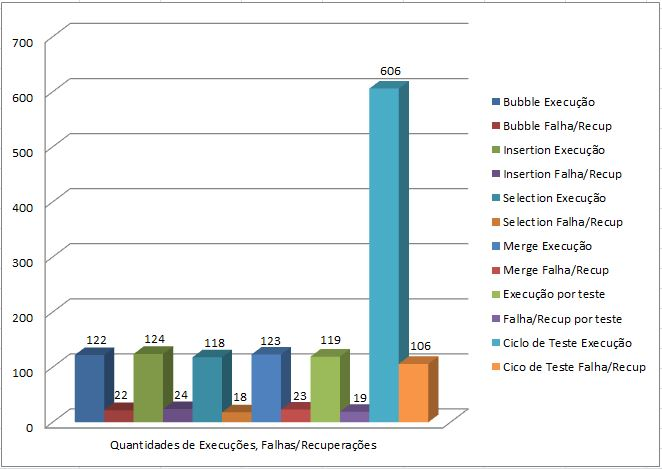
\includegraphics[width=0.9\textwidth]{figuras/testeFaultRecovery.jpg}
	\caption[Resultados Obtidos da Biblioteca \textit{FaultRecovery}]{Nesta Figura é mostrada a quantidade de execuções e falhas de cada algoritmo, inclusive de cada ciclo de teste. Por exemplo, a primeira coluna, da esquerda para e direita, representa o número de execuções do algoritmo \textit{bubble sort}, pode-se perceber que embora tenham sido executados cem ciclos de teste, o algoritmo foi executado cento e vinte e duas vezes. Em contra partida, na segunda coluna, que representa a quantidade de vezes em que um ponto de recuperação do \textit{bubble sort} foi executado, o \textit{firmware} reinicializou e executou o ponto de recuperação do \textit{bubble sort} vinte e duas vezes.}
	\label{Img:testeFaultRecovery}	
	%width=0.5\textwidth (Tamanho da Imagem)
\end{figure}

\newpage
\section{Injeção de Falhas com a Biblioteca \textit{FaultInjector}}

Esta Seção mostra o resultado de injeção de falhas na memória \textit{flash} do microcontrolador \textit{mbed} LPC1768. A injeção de falhas na memória \textit{flash} sorteou um setor aleatório para injetar uma quantidade predefinida de falhas, que podem variar de 256, 512, 1024 ou 4096 bytes. Na Figura \ref{Img:injecaoFlash} é exibido um teste em que foram injetadas 256 bytes de falhas no setor 25, que foi sorteado aleatoriamente pelo injetor de falhas. O endereço de memória do setor sorteado em hexadecimal inicia em 0x00058000 e termina em 0x0005FFFF. Pode-se perceber que os bytes dos endereços de memória do setor 25 (0x00058000 até 0x000580F0) foram alterados.

\begin{figure}
	\centering
	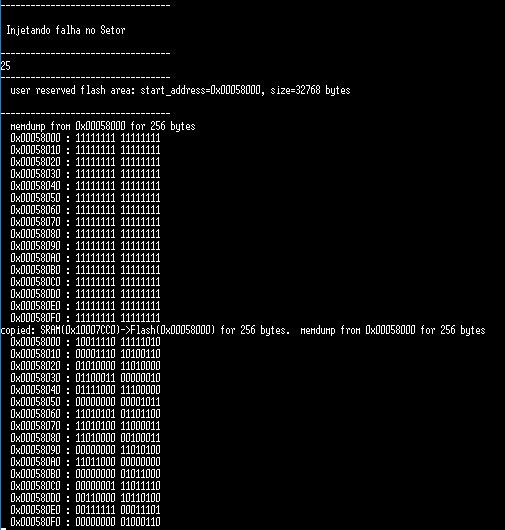
\includegraphics[width=0.9\textwidth]{figuras/injecaoFlash.jpg}
	\caption[Injeção de Falhas na Memória \textit{Flash}]{Nesta Figura é mostrado o setor da memória \textit{flash} soteado pelo injetor de falhas e os endereços desse setor. Além de mostrar como os bits se encontravam antes de serem modificados, assim como também pode ser visualizada a modificação desses bits.}
	\label{Img:injecaoFlash}	
	%width=0.5\textwidth (Tamanho da Imagem)
\end{figure} % Resultados
	%====================================================================================================
%----------------------------------------------------------------------------------------------------
% Autor				: Vagner da Silva Bezerra
%----------------------------------------------------------------------------------------------------
% Data de criação	: 10 de Outubro de 2016
%====================================================================================================

\chapter{Conclusão} \label{cap:conclusao}

Neste trabalho a biblioteca \textit{FaultRecovery} foi modificada para ser utilizada por usuários que queiram modularizar seu código, separando os estados de seu \textit{firmware} por responsabilidades. A ideia e parte do código da biblioteca \textit{FaultRecovery} está sendo utilizada pelo projeto de extensão Coxim Robótica sediado na UFMS - Campus Coxim. O alunos estão programando um robô seguidor de linha, no qual são necessários alguns estados para que o carrinho desempenhe suas funções, como desviar de um obstáculo ou seguir em frente. Cada aluno do projeto é responsável pela implementação de um estado da máquina de estados do carrinho seguidor de linha.  

Foram implementados testes com a biblioteca \textit{FaultRecovery} e sem ela. Foi constatado que na implementação sem a biblioteca o \textit{firmware} falhou e dessa forma não continuou a sequência de sua máquina de estados, pois não existia nenhum mecanismo de recuperação de falhas. No entanto nos testes realizados com a \textit{FaultRecovery}, em todas as vezes que o \textit{firmware} reiniciava, um ponto de recuperação era executado, mantendo a sequência original da máquina de estados. Existem pesquisas na área de semicondutores e na área de robótica que mostram os ruídos nos sensores como um problema comum que pode afetar a eficácia de algoritmos. Para contornar esse problema foi implementada neste trabalho a redundância de dados por meio da classe \textit{TData}, que se mostrou eficaz em manter a integridade dos dados, protegendo as informações que por ventura venham a ser modificadas por falhas. A \textit{TData} foi acrescentada à biblioteca \textit{FautRecovery}, sendo assim o usuário que utilizá-la poderá criar pontos de recuperação e separar o seu código, também poderá proteger dados importantes de seu \textit{firmware}. Cabe observar que a biblioteca se mostrou eficaz na resolução do problema, pois em todos os testes o \textit{firmware} tolerou 100\% das falhas injetadas.

No entanto, a biblioteca adiciona um custo de desempenho no tempo de processamento, uma vez que toda a operação de leitura e escrita em uma variável, feita pela classe \textit{TData}, é custosa devido a execução de um esquema de votação usado para definir o valor correto permanecente em todas as cópias. Porém, isso já era esperado, ainda sim o uso da biblioteca se torna mais vantajoso pelo fato de a maioria das aplicações embarcadas não terem como fator principal o tempo de execução, exceto algumas aplicações de tempo real. Mas nestes casos são utilizados microcontroladores com um maior poder de processamento. 

A biblioteca \textit{FaultInjector} também foi modificada neste trabalho, agora é possível injetar falhas na memória \textit{flash}. No teste realizado, mostrou-se os bits armazenados em determinado setor da memória \textit{flash} antes e depois da injeção de falhas. Com isso foi possível visualizar os bits sendo alterados. Além disso, também foi incluído um mapeamento de memória que possibilita a utilização do injetor de falhas em modelos pertencentes a família \textit{mbed} LPC176X. Porém só foi possível testar o mapeamento de memória no modelo 1768, pois era o único microcontrolador disponível para este trabalho. O mapeamento funcionou para o modelo disponível e foi possível injetar falhas nos endereços de memória disponíveis no mapeamento. Tanto a biblioteca \textit{FaultRecovery}, quanto a \textit{FaultInjector} estão disponíveis no \textit{github}, nos endereços \url{https://github.com/cleitonalmeida1/FaultRecovery} e \url{https://github.com/cleitonalmeida1/FaultInjector}

Os resultados apresentados neste trabalho se mostraram bons, devido ao bom funcionamento das bibliotecas e a eficácia em solucionar problemas ocasionados por falhas. Conforme Johnson \cite{Johnson:1984}, tolerância a falhas é a propriedade que permite a um sistema continuar funcionando adequadamente, mesmo que num nível reduzido, após a manifestação de falhas em alguns de seus componentes.

\section {Contribuições deste Trabalho}

Uma arquitetura de desenvolvimento de aplicações embarcadas por meio de uma máquina de estados. Essa arquitetura está sendo utilizada pelos alunos do projeto de extensão Coxim robótica sediado na UFMS - campus Coxim. Em uma breve conversa  com os integrantes do projeto, que antes programavam em um mesmo computador, informaram que o desenvolvimento do programa está mais rápido pois agora eles podem trabalhar em mais de um estado ao mesmo tempo.

\section{Dificuldades Encontradas}

No início da implementação encontrou-se bastante dificuldade para se adaptar a uma linguagem de programação diferente de java. Embora elas sejam parecidas, a preparação do ambiente de desenvolvimento é totalmente diferente. Foram encontradas algumas dificuldades para configurar a IDE e o compilador c++ no windows 10. Além do tempo de estudo da linguagem que levou mais de 15 dias para adaptação. Por ser uma linguagem de ampla utilização, existem muitos fóruns de dúvidas que ajudaram durante o desenvolvimento. 

\section{Trabalhos Futuros} \label{Sec:TrabalhosFuturos}

\begin{itemize}

\item Testar o mapeamento de memória incluído na biblioteca \textit{FaultInjector} para outros modelos além do modelo \textit{mbed} LPC1768.

\item Salvar as cópias utilizadas pela classe \textit{TData}, para se ter redundância de dados, em outras regiões de memória. Atualmente as cópias estão sendo salvas na região de memória reservada ao usuário, mas futuramente poderá ser salva na região destinada aos periféricos internos do microcontrolador. 

\item Aperfeiçoar a biblioteca \textit{FaultRecovery} e a classe \textit{TData} para diminuir o tempo de processamento em uma aplicação embarcada.

\item Explorar a injeção de falhas na memória \textit{flash}, implementando um \textit{firmware} e injetando falhas enquanto ele está em execução.

\end{itemize}
 % Conclusão
	
	\pagestyle{empty}
	%====================================================================================================
%----------------------------------------------------------------------------------------------------
% Autor				: Vagner da Silva Bezerra
%----------------------------------------------------------------------------------------------------
% Data de criação	: 10 de Outubro de 2016
%====================================================================================================


%\phantomsection
%\cleardoublepage
\bibliographystyle{abnt}
\renewcommand\bibname{Referências}
%\bibliographystyle{apalike} 
%\bibliographystyle{ieeetr} % Ordena por ordem de aparição.  
%\bibliographystyle{abbr} % Ordena por ordem alfabetica com nomes abreviados.
%\bibliographystyle{plain} % Ordena por ordem alfabetica com nomes por extenso.
%\bibliography{Referências} % commented if *.bbl file included.
\bibliography{referencias} % commented if *.bbl file included.
\addcontentsline{toc}{chapter}{Referências}
\cleardoublepage
%\thispagestyle{empty} % Referências Bibliográficas
	%====================================================================================================
%----------------------------------------------------------------------------------------------------
% Autor				: Vagner da Silva Bezerra
%----------------------------------------------------------------------------------------------------
% Data de criação	: 10 de Outubro de 2016
%====================================================================================================

%\hypertarget{apendice}{}
%\bookmark[dest=apendice]{Apêndice}
\chapter*{Apêndice} \label{App:ApendiceA}
\addcontentsline{toc}{chapter}{Apêndice}
\appendix

%\includepdf[pages={1-17}]{apendice.pdf}
\includepdf[pages={1-17},pagecommand={\thispagestyle{plain}}]{apendice.pdf}
%\includepdf[pages=-,pagecommand={\thispagestyle{plain}}]{GameTheoryTutorial10.pdf}

	%====================================================================================================
%----------------------------------------------------------------------------------------------------
% Autor				: Vagner da Silva Bezerra
%----------------------------------------------------------------------------------------------------
% Data de criação	: 10 de Outubro de 2016
%====================================================================================================

%\hypertarget{anexo}{}
%\bookmark[dest=anexo]{Anexo}
\chapter*{Anexo} \label{App:AnexoA}
\addcontentsline{toc}{chapter}{Anexo}
\appendix

%\includepdf[pages={1-17}]{anexos.pdf}

\end{document}